\documentclass[12pt]{article}
\usepackage[a4paper]{subook}

\providecommand{\tightlist}{%
  \setlength{\itemsep}{0pt}\setlength{\parskip}{0pt}}

\usepackage{minted}
\usepackage{xcolor}

\definecolor{Mycolor1}{HTML}{6a510f}
\definecolor{Mycolor2}{HTML}{0f536a}


\hypersetup{
    colorlinks=true,
    linkcolor=Mycolor2,
    filecolor=magenta,
    urlcolor=Mycolor1
}

\usemintedstyle{tango}

\begin{document}


Copyright © 2019 Зак Голлвитцер
Copyright © 2021 Евгений Черкашин

\clearpage

\setcounter{tocdepth}{3}
\tableofcontents

\clearpage

\section*{Предисловие от составителя пособия}
% \addcontentsline{toc}{section}{Предисловие от составителя пособия}

Данный методический материал создан путем перевода текста, опубликованному в виде \href{https://zachgoll.github.io/blog/2019/bash-essentials/}{данного поста} его первоначальным автором Заком Голлвитцером (Zach Gollwitzer). Перевод осуществлен при помощи системы CAT (Computer Aided Translation) OmegaT и единственного на данный момент бесплатного сервера \href{https://mymemory.translated.net/}{MyMemory}. Автор перевода, таже по совмещению являющийся соавтором данного пособия, подверг первоначальный стиль существенной переработке, стараясь сделать его в большей степени соответствующим к стандартам публикации учебных пособий в образовательной системе РФ. Не все конечно удалось, поэтому оставлю проект открытым к редактированию на сайте \href{https://www.overleaf.com/project/602cc04c00be7fbbe118f862}{Overleaf} для дальнейшего редактирования и совершенствования стиля.

Пособие состоит из трех разделов, первые два -- собственно адаптация оригинального текста, в который не добавлялся новый материал, третий раздел содержит методический материал для выполнения лабораторной работы, направленной на развитие навыков разработки скриптов (сценариев) в командной оболочке bash. Представленный материал далеко не полностью покрывает такою обширную область разработки сценариев bash, но что необходимо выделить как положительный момент -- практическая направленность. Зак Голлвитцер на собственном опыте показывает решение ряда задач, с которым он регулярно сталкивается в своей деятельности, в том числе администрирование собственного домашнего компьютера с операционной системой Linux/Mac. Зак учит читателя не только основным командам, запускаемым из оболочки, но и как искать справочную по ним информацию: использовать программу man и поисковую систему Google.

Материал разработан для студентов, изучающих программирование и администрирование в рамках специальностей 09.03.01 -- <<Информатика и вычислительная техника>> и 09.03.02 -- <<Информационные системы и технологии>>, вероятно, может быть использована в других направлениях обучения.

\vspace{3em}
\begin{flushright}\it
  Канд. техн. наук, доцент ИрНИТУ, Е.А.Черкашин
\end{flushright}

\clearpage

\hypertarget{Environment-variables}{%
\section{\texorpdfstring{\protect\hyperlink{Environment-variables}{}Базовый уровень}{Базовый уровень}}\label{Environment-variables}}

Перед тем, как начать изучать командную оболочку bash, есть несколько
важных концепций, помимо основных команд, необходимых к изучению. Перед
освоением основ и управления правами пользователя необходимо
изучить переменные среды, псевдонимы и некоторые более сложные команды,
относящиеся к сетям, управлению процессами, ssh и сценариям.

Переменная среды может быть глобальной или локальной. Глобальная
переменная среды -- это переменная, которая устанавливается при
инициализации оболочки и может использоваться во всех дочерних скриптах.
Сеансовая (локальная) переменная среды -- это переменная, которая
устанавливается во время конкретного сеанса оболочки и стирается при его
закрытии. Чтобы создать сеансовую переменную среды надо export-ировать
ее в текущую оболочку.

\begin{minted}{bash}
export MY_VARIABLE="значение"
\end{minted}

Ее можно использовать пока оболочка все еще открыта.

\begin{minted}{bash}
echo $MY_VARIABLE # значение
\end{minted}

Как только вы закроете оболочку, переменная более не будет доступна.
Чтобы сделать переменную глобальной, ее помещают в один из файлов
конфигурации bash. Рекомендуется поместить ее в
\texttt{\textasciitilde{}/.profile}-файл.

\begin{minted}{bash}
# ~/.profile

export GLOBAL_VARIABLE="значение"
\end{minted}

Чтобы увидеть все переменные текущего сеанса (как локальные, так и
глобальные), можно запустить команду

\begin{minted}{bash}
env
\end{minted}

\hypertarget{Shell-Variables}{%
\subsection{\texorpdfstring{\protect\hyperlink{Shell-Variables}{}Переменные
среды и оболочки}{Переменные среды и оболочки}}\label{Shell-Variables}}

Пользователи bash часто путаются, говоря о переменных \emph{среды} и
переменных \emph{оболочки}. Независимо от того, является ли переменная
среды локальной или глобальной, все сценарии, запущенные в этом сеансе
bash, будут иметь доступ к переменной. С переменной оболочки все не так:
другие сценарии не будут иметь к ней доступа. Ниже показано, как
объявляются переменные оболочки.

\begin{minted}{bash}
MY_SHELL_VARIABLE="значение"

echo $MY_SHELL_VARIABLE  # значение
\end{minted}

Эта переменная не будет доступна ни одному сценарию, пока не будет
экспортирована и не сделана переменной среды.

\begin{minted}{bash}
export MY_SHELL_VARIABLE
\end{minted}

\hypertarget{PATH-variable}{%
\subsection{\texorpdfstring{\protect\hyperlink{PATH-variable}{}Переменная
PATH}{Переменная PATH}}\label{PATH-variable}}

Самая важная глобальная переменная среды, которую очень часто
устанавливают, - это переменная \texttt{PATH}. Она сообщает оболочке
bash, где искать исполняемые файлы и сценарии. Оболочка перебирает
каталоги, перечисленные в переменной \texttt{PATH}, пытаясь найти
программу, которую требуется запустить. Вот пример установки переменной
PATH.

\begin{minted}{bash}
export PATH=/usr/local/bin:/usr/bin:/bin
\end{minted}

В этом примере, если пользователь хочет запустить программу
\texttt{cat}, bash сначала будет искать ее в директории
\texttt{/usr/local/bin}. Если он не найдет его там, он перейдет в
\texttt{/usr/bin}, и, наконец, в \texttt{/bin}. Если вам нужно изменить
путь, вы можете обновить его в своем
\texttt{\textasciitilde{}/.profile}:

\begin{minted}{bash}
export PATH=/home/zach/script-location:$PATH
\end{minted}

Команда добавляет директорий \texttt{/home/zach/script-location} в
начало списка \texttt{PATH}. Если вы хотите добавить новый директорий
его в конец списка, то это делается следующим образом:

\begin{minted}{bash}
export PATH=$PATH:/home/zach/script
\end{minted}

Теперь можно создавать специальные библиотеки сценариев и запускать их
автоматически из директориев, указанных в PATH. Теперь создадим каталог
в домашней папке, который будет хранить все наши скрипты.

\begin{minted}{bash}
cd ~
mkdir bin
touch bin/my-simple-script
\end{minted}

Теперь надо добавить этот текст в \texttt{my-simple-script}.

\begin{minted}{bash}
#!/bin/bash
echo "Бесполезный скрипт, предназначенный исключительно для демонстрации."
\end{minted}

Теперь устанавливаем флаг, позволяющий запускать скрипт.

\begin{minted}{bash}
chmod 775 my-simple-script
\end{minted}

Теперь надо добавить новый каталог \texttt{/bin} к нашей PATH.
Редактируем \texttt{\textasciitilde{}/.profile} (или другой, где
определяется переменная \texttt{PATH}), добавляем следующую строку.

\begin{minted}{bash}
export PATH=$PATH:~/bin
\end{minted}

Наконец, активируем изменения из
\texttt{source\ \textasciitilde{}/.profile} в текущем сеансе.

\begin{minted}{bash}
source ~/.profile
\end{minted}

Теперь можно запускать свой скрипт из командной строки, указав его имя.

\begin{minted}{bash}
./my-simple-script
# Бесполезный скрипт, предназначенный исключительно для демонстрации.
\end{minted}

\hypertarget{Common-Commands}{%
\subsection{\texorpdfstring{\protect\hyperlink{Common-Commands}{}Основные
команды}{Основные команды}}\label{Common-Commands}}

Помимо основных команд, таких как \texttt{cd}, \texttt{ls},
\texttt{mkdir}, \texttt{touch} и т.д., есть небольшой список команд,
которые в bash используются на регулярной основе.

\begin{itemize}
\tightlist
\item
  grep
\item
  awk/sed
\item
  less
\item
  Команды find и exec
\item
  gunzip
\item
  tar
\end{itemize}

\hypertarget{grep}{%
  \subsubsection{\texorpdfstring{\protect\hyperlink{grep}{}Программа grep}{Программа grep}}\label{grep}}

Grep - это инструмент, который ищет шаблоны или слова в одном или
нескольких файлах. Программа существует в двух версиях: BSD и GNU. В
системах Mac используются BSD-вариянт, системы с Linux - GNU. В
рассмотренных далее примерах различия между этими версиями не заметны,
но если вдруг в той или иной операционной системе что-то пойдет не по
плану, надо уточнить свойства конкретной версии. Например, могут
отличаться определенные типы регулярных выражений.

Grep можно воспринимать как инструмент поиска, встроенный в командную
строку. В современных средах программирования (текстовых редакторах)
есть много инструментов поиска. Например, в Visual Studio Code Editor
можно использовать строку поиска для того, чтобы искать в файлах проекта
определенное слово или даже соответствие регулярному выражению (рис.~\ref{fig:vscodesearch}). В
результате редактором перечисляются файлы, в которых было найдено
выражение, указывается строка, где оно было найдено и т.д.
\begin{figure}[tbh]\centering

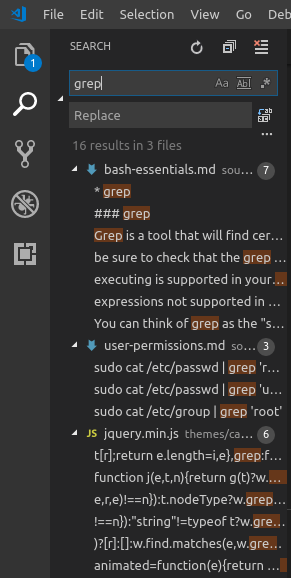
\includegraphics[width=0.5\linewidth]{blog/2019/bash-essentials/vscode-search.png}

\caption{Поиск строки в VSCode}
\label{fig:vscodesearch}
\end{figure}
В этом примере, автор искал в своем блоге слово <<grep>> и нашел его в
трех разных файлах. Но что делать, если VSCode недоступен? Такое может
быть, если вы управляете удаленной машины, или, просто, к этой
удивительной функции поиска нет доступа? В этом случае grep просто
незаменим. Основной синтаксис для использования grep следующий:

\begin{minted}{bash}
grep [все опции и ключи здесь] "текст, который ищется" <имя-файла-где-ищем>
\end{minted}

Например, попробуем найти имя пользователя в файле \texttt{/etc/passwd}
(где хранятся все пользователи в системе).

\begin{minted}{bash}
# Необходимо использовать sudo, потому что этот файл защищен
# Флаг (ключ) -i переводит поиск в режим игнорирования размера букв
sudo grep -i "zach" /etc/passwd

# zach:x:1000:1000:Zach,,,:/home/zach:/bin/bash
\end{minted}

Хотя это руководство не преследует целью детально описать регулярные
выражения, все же рассмотрим простой пример. Например, чтобы найти всех
пользователей, имена которых состоят из трех символов, надо использовать
флаг \texttt{-E}, включающий режим <<расширенных регулярных выражений>>.

\begin{minted}{bash}
sudo grep --color -E "^[a-z]{3}:" /etc/passwd

# Результат ---
#bin:x:2:2:bin:/bin:/usr/sbin/nologin
#sys:x:3:3:sys:/dev:/usr/sbin/nologin
#man:x:6:12:man:/var/cache/man:/usr/sbin/nologin
#irc:x:39:39:ircd:/var/run/ircd:/usr/sbin/nologin
#gdm:x:121:125:Gnome Display Manager:/var/lib/gdm3:/bin/false
\end{minted}

Слова \texttt{bin}, \texttt{sys}, \texttt{man}, \texttt{irc} и \texttt{gdm} - это трехбуквенные имена пользователей. Если результат выдается в монохромном
режиме, можно его раскрасить, добавив флаг \texttt{цвета}.

Еще один способ использования grep - в режиме фильтра вывода другой
команды. Результат (stdout), выдаваемый одной командой, можно передать
на вход (stdin) grep. Теперь то, что мы делали выше, можно сделать
по-другому:

\begin{minted}{bash}
sudo cat /etc/passwd | grep --color -E "^[a-z]{3}:"
\end{minted}

Таким образом, утилита \texttt{grep} полезна для быстрого поиска, если у
вас нет доступа к текстовому редактору, например, VSCode, или нет
желания ждать, пока он загрузится.

\hypertarget{awk-and-sed}{%
\subsubsection{\texorpdfstring{\protect\hyperlink{awk-and-sed}{}Утилиты
awk и sed}{Утилиты awk и sed}}\label{awk-and-sed}}

В настоящее время, \texttt{awk} и \texttt{sed} являются предметом споров
и обсуждений, и в этом разделе попробуем разъяснить \emph{почему} это
происходит, ну и покажем основные формы их использования. Причина
стопорит в том, что сейчас существуют лучшие альтернативы. Обе
программы обрабатывают тексты, они могут находить \emph{и} заменять
части одного файла или наборы файлов.

Программа sed является редактором текстового потока (Stream EDitor):
производит посимвольный просмотр файла, и не считается полноценным
языком программирования. Он отлично подходит для простых операций типа
<<найти и заменить>> над одним или несколькими файлами. Опять же, эта
операция элементарно реализуется в текстовых редакторах типа VSCode, но
иногда к редактору нет доступа, или есть необходимость выполнения
операции над группой файлов, в скрипте.

Язык awk считается достаточно полным языком программирования и больше ориентирован на табличные текстовые данные, где
столбцы разделены специальными символами, например формата CSV (Comma
Separated Values). Например, \texttt{awk} хорошо разбивает файл csv или
файл, разделенный пробелами, поскольку он обрабатывает входной файл
построчно, а не посимвольно.

Проблема с этими программами заключается в том, что все, что можно
сделать, комбинируя sed или awk, можно реализовать в языках Perl или
Python в более простой. Бесспорно, Perl и Python являются гораздо более
удобными языками реализации сценариев. В защиту утилит высказывают, что
sed и awk обладают превосходной производительностью на определенных
задачах, но практика показывает, что Perl или Python все же лучшие
решения.

Однако в некоторых задачах администрирования обрабатывать тексты
приходится при помощи sed и awk, так как, опять же, может не быть
доступа к Python или Perl. Теперь возникает вопрос: в чем разница между
этими утилитами? Когда надо использовать sed, а когда awk? Вот несколько
простых правил:

\begin{itemize}
\tightlist
\item
  Для простых текстовых преобразований (например, найти/заменить),
  используйте sed.
\item
  Для простых преобразований формата используйте awk
\item
  Для сложных преобразований формата и текста используйте awk
\end{itemize}

Рассмотрим примеры каждой из задач, покажем использование обоих
инструментов. Начнем с простой операции по поиску/замене при помощи sed.
В качестве обрабатываемого текста использован образец файла от Apple
Inc., данные по акциям за последние 3 месяца, файл \texttt{AAPL.csv}.
Исходные данные:

\begin{minted}{bash}
Date,Open,High,Low,Close,Adj Close,Volume
2018-11-06,201.919998,204.720001,201.690002,203.770004,203.061493,31882900
2018-11-07,205.970001,210.059998,204.130005,209.949997,209.219986,33424400
2018-11-08,209.979996,210.119995,206.750000,208.490005,208.490005,25362600

... пропущены аналогичные записи ...

2019-02-04,167.410004,171.660004,167.279999,171.250000,171.250000,31495500
2019-02-05,172.860001,175.080002,172.350006,174.179993,174.179993,36066500
\end{minted}

Для замены всех запятых с пробелами удобно использовать sed.

\begin{minted}{bash}
sed 's/,/ /g' AAPL.csv
\end{minted}

\begin{minted}{bash}
Date Open High Low Close Adj Close Volume
2018-11-06 201.919998 204.720001 201.690002 203.770004 203.061493 31882900
2018-11-07 205.970001 210.059998 204.130005 209.949997 209.219986 33424400
2018-11-08 209.979996 210.119995 206.750000 208.490005 208.490005 25362600

... пропущены аналогичные записи ...

2019-02-04 167.410004 171.660004 167.279999 171.250000 171.250000 31495500
2019-02-05 172.860001 175.080002 172.350006 174.179993 174.179993 36066500
\end{minted}

Будет распечатан результат преобразования из sed. Если добавить флаг -i,
то sed будет редактировать исходный файл (in-place).

\begin{minted}{bash}
sed -i 's/,/ /g' AAPL.csv
\end{minted}

Теперь, когда у нас есть файл, где столбцы разделены пробелами. Теперь
можно использовать \texttt{awk} для вычисления агрегированных значений.
В этих данных в текущем их состоянии цена акций задается в нескольких
столбцах (open, high, low, close, adjusted), что можно подправить.
Например, выделим цены в колонках open и volume по датам (date). Для
выделения этих столбцов используем awk.

\begin{minted}{bash}
awk -F " " ' BEGIN { print "Date\t\tPrice\t\tVolume" }; NR > 1 \
     { print $1 "\t" $2 "\t" $7 } ' AAPL.csv
\end{minted}

\begin{minted}{bash}
Date            Price           Volume
2018-11-06      201.919998      31882900
2018-11-07      205.970001      33424400
2018-11-08      209.979996      25362600

... пропущены аналогичные записи ...

2019-02-04      167.410004      31495500
2019-02-05      172.860001      36066500
\end{minted}

На первый взгляд команда выглядит слишком сложной для изучения, но
проведем некоторый ее обзор. Основы синтаксиса awk можно узнать, сделав
соответствующие запросы к поисковой системе Google, также можно найти
примеры решения конкретных задач.

Программа awk - это больше язык программирования, а не команда обработки
текста. Чтобы узнать, что означает вышеупомянутая команда, сохраним ее в
файл, что удобнее для обучения. Создадим файл \texttt{awk-example.sh} и
поместим туда вышеупомянутую команду, отформатируем текст программы.

\begin{minted}{bash}
# Это комментарий в программе awk
# Перед тем, как непосредственно перейти к обработке текста
# установим переменную FS (задает символ-разделитель колонок),
# переменную OFS (символ-разделитель в выходных данных),
# и затем распечатаем заголовок текста в порождаемом результате.
BEGIN {
        # Обратите внимание, каждая строка заканчивается символом ";",
        # что приближает этот скрипт к языку программирования C.
        FS=" ";
        OFS="\t";
        print "Date\t\tPrice\t\tVolume";
};

# NR > 1 означает, что надо распечатать значения из строк,
# номера которых больше 1.
#   Другими словами, мы пропускаем первую строку.
NR > 1 {
        # Выводим первое, второе и седьмое значение их каждой строки.
        print $1, $2, $7;
};
\end{minted}

Запуск программы осуществляется так:

\begin{minted}{bash}
# Выводится то же самое, что в результате запуска
# awk -F " " ' BEGIN { print "Date\t\tPrice\t\tVolume" }; NR > 1 \
  { print $1 "\t" $2 "\t" $7 } ' AAPL.csv
# Загружаем программу из awk-example.sh, применяем ее к файлу AAPL.csv.csv
awk -f awk-example.sh AAPL.csv
\end{minted}

Как можно было заметить, в awk есть встроенные переменные, включая
\texttt{FS} (символ-разделитель входного файла), \texttt{OFS}
(символ-резделитель для выходного файла), \texttt{NR} (номер строки).
Дркгие переменные можно найти
\href{https://www.tutorialspoint.com/awk/awk_built_in_variables.htm}{здесь}.
Можно использовать переменные вместо задания флагов в командной строке.
Например, вместо флага \texttt{-F\ "\ "} можно установить
соответствующее значение переменной \texttt{FS} в программе awk.

Обучение всем возможностям \texttt{awk} займет гораздо больше времени,
чем это оправдано для данного руководства, но освоив основу синтаксиса,
проще изучить все остальное. В конечном счете, каждая awk команда есть
наборы ключевых слов и команд формирования выходных данных. Команда,
которую только что запустили, полностью показана ниже.

\begin{minted}{bash}
# awk executable | Options | Keyword  | What to print based on keyword
#    Keyword   What to print based on keyword | file to run
awk               -F " " '   BEGIN    { print "Date\t\tPrice\t\tVolume" }; \
     NR > 1    { print $1 "\t" $2 "\t" $7 } '   aapl.csv
\end{minted}

Программа awk обладает большим набором функций, включая редактирование
файлов. Хороший учебник по программе находится
\href{https://likegeeks.com/awk-command/}{здесь}.

На самом деле для более сложных задач нет необходимости в е изучении sed
и awk. Языки Perl/Python также позволяют обрабатывать текст, при этом
использовать более простой синтаксис. Тем не менее знание основ
использования этих команд может значительно ускорить ваш рабочий процесс
при решении простых задач, которые периодически возникают. Они также
полезны когда вы пишете сценарий для bash, где нужно как-то
редактировать текст или изымать оттуда информацию. Было бы неудобно
вручную останавливать сценарий bash, запускать скрипт python, а затем
перезапускать сценарий снова. Утилиты sed и awk предоставляют
возможность избегать такого варианта обработки информации.

\hypertarget{Less}{%
\subsubsection{\texorpdfstring{\protect\hyperlink{Less}{}Программа
Less}{Программа Less}}\label{Less}}

Программа less одной из тех утилит командной строки, которую вы
наверняка не используете, а должны были бы. Программа позволяет
просматривать текстовые денные, интерактивно прокручивая строки на
экране при помощи клавиатуры. Программа проста в использовании, и
работает аналогично редактору vim. Существует два способа использования
less:

\begin{minted}{bash}
# Передача выходных данных в less из другой программы
cat some-large-file.txt | less

# Использование less напрямую
less some-large-file.txt
\end{minted}

В запущенной программе есть замечательная функция - h. Нажатие
\texttt{h} открывает панель помощи, где отображаются все возможные
интерактивные команды. Приведем самые полезные.

\begin{itemize}
\tightlist
\item
  Для прокрутки на одну строку, жмите \texttt{k} (как в vim)
\item
  Для прокурутки на одну линию вниз, жмите \texttt{j} (как в vim)
\item
  Чтобы перейти в конец файла, жмите \texttt{G}
\item
  Чтобы перейти к началу файла, жмите \texttt{g}
\item
  Для поиска <<текста>>, наберите \texttt{/текст} (поиск по тексту вниз)
  или '?
\item
  Для продвижения вниз на страницу, жмите \texttt{f} или <<пробел>>
\item
  Чтобы пролистать на страницу вверх, жмите \texttt{b}
\end{itemize}

Так же, как grep, awk и sed, прокрутка и поиск в тексте удобнее делать в
текстовых редакторах, например, VSCode. Если есть возможность
используйте редактор. Использование команды \texttt{less} удобно, если
редактор недоступен или медленнее, чем нужно, грузится.

\hypertarget{find-and-exec}{%
\subsubsection{\texorpdfstring{\protect\hyperlink{find-and-exec}{}Команды
find и exec}{Команды find и exec}}\label{find-and-exec}}

На первый взгляд, команда find очень сильно похожа на grep, но ее
использование охватывает решение других задач. Программа поиска
необходима, если вы хотите искать файлы с определенными свойствами во
всей файловой системе. Напомним, что grep ищет текст в файле или в
тексте-результате предыдущей команды, find ищет именно файлы в файловой
системе. Почему он полезен? Команда find возвращает полный путь до файла
по имени и или атрибутам: запускаемый, читаемый, редактируемый и т.д.
Например, давным-давно вы установили нужную вам версию Python и не
можете вспомнить, куда вы скачали архив его исходников. Это обычная
проблема - порождать версии Python на вашей машине, которые конфликтуют
друг с другом. Кроме того, часто надо полностью удалить все версии
Python с компьютера. Другие виды использования find включают:

\begin{itemize}
\tightlist
\item
  Найти все файлы .png на компьютере
\item
  Найти все документы, измененные некоторым пользователем за последние 7
  дней
\item
  Найти файлы, имеющие определенный набор разрешений (permission set)
\end{itemize}

Как видно, возможности \texttt{find} практически безграничны, и если
использовать ее весь потенциал, можно решить много разных задач, включая
те, до которых вы раньше не додумывались. Вот простой пример:

\begin{minted}{bash}
find / -type f -size +1G
\end{minted}

Эта команда перечислит все файлы на компьютере, размер которых больше 1
гигабайта. Если у вас мало места на дисках, эта команда поможет найти те
файлы, которые занимает недоступное пространство на вашем компьютере.

Основным форматом использования команды find является

\begin{minted}{bash}
find <директорий, где производить поиск> [флаги] <имя файла, который ищем>
\end{minted}

Вот несколько полезных и часто используемых команд:

\begin{minted}{bash}
# Найти все .jpg-файлы на компьютере
find / -type f "*.jpg"

# Найти все файлы, измененные за прошедшие сутки
find / -type f -mtime 1

# Найти все файлы, которые принадлежат пользователю zach
find / -type f -user zach

# Найти все файлы с кодом разрешений 777
find / -type f -perm 777

# Найти все файлы, имена которых начинаются со слова config
find / -type f -name "config*"
\end{minted}

Это всего лишь несколько из тысячи других функций программы. Кроме того,
используя команду \texttt{exec}, \texttt{find} переходит на новый
уровень. Вместо того чтобы просто искать файлs, можно также выполнять с
ними другие операции. Хотя это очень здорово, но и очень опасно, если не
соблюдать осторожность, ясно представлять, что будет происходить во
время исполнения команды. Функция exec позволяет запускать другие
команды над найденным \texttt{find} файлом. Если вы объедините
\texttt{find} и \texttt{rm}, запущенной при помощи \texttt{exec}, вы
можете удалить найденные файлы. Поэтому, прежде чем запускать такие
конструкции, проверяйте все десять раз!

Пусть есть простая команда на основе find, которая ищет все файлы .jpg
домашнем каталоге.

\begin{minted}{bash}
find ~/ -type f -name "*.jpg"
\end{minted}

Если есть необходимость скопировать все совпадения в папку
\texttt{\textasciitilde{}/pictures-backup}, добавляем команду exec.

\begin{minted}{bash}
find ~/ -type f -name "*.jpg" -exec '{}' ~/pictures-backup \;
\end{minted}

Наверное интересно, что такое
\texttt{\textquotesingle{}\{\}\textquotesingle{}} и
\texttt{\textbackslash{};}, что это за элементы, использованные в
команде. Пользуясь новыми навыками, вы можете посмотреть дополнительную
информацию о \texttt{exec}, перенаправив вывод - страницу man в less и
выполнив поиск по слову «exec».

\begin{minted}{bash}
man find | less
/-exec
п # повторяет поиск для строки -exec и находит следующее его вхождение
\end{minted}

На этих страницах руководства видно, что
\texttt{\textquotesingle{}\{\}\textquotesingle{}} указывает место, куда
подставлять найденные файлы, и \texttt{\textbackslash{};} - это символ,
указывающий границу команды для запуска \texttt{exec}. Обратная косая
черта -- это механизм <<избавления от лишних проблем>>. Можно просто
использовать \texttt{\textquotesingle{};\textquotesingle{}}.

После выполнения этой команды, все изображения jpg из домашнего каталога
будут скопированы в централизованное хранилище резервных копий! Теперь
вы ведите, как крута эта команда!

\hypertarget{tar-gzip-gunzip}{%
\subsubsection{\texorpdfstring{\protect\hyperlink{tar-gzip-gunzip}{}Команды
tar, gzip, gunzip}{Команды tar, gzip, gunzip}}\label{tar-gzip-gunzip}}

Эти утилиты не имеют какого-то сложного набора функций и используются
для сжатия и распаковки файлов. Часто, при загрузке релиза программы или
серии больших файлов или изображений, мы можем получить их в формате
\texttt{.tar}, \texttt{.gz}, или даже \texttt{.tar.gz}. \texttt{tar} и
\texttt{gz} - это разные программы. \texttt{tar} - это формат архива
набора файлов, а \texttt{gz} - это формат сжатия информации. В
большинстве случаев можно использовать файловый менеджер компьютера, он
способен обрабатывать эти форматы, но иногда нужно распаковать файл в
командной строке (например, на удаленном сервере). Вот самые
распространенные команды.

\begin{minted}{bash}
# Создяние .tar-архива
# c - создать, v - подробный вывод, f - формат tar
tar cvf archive.tar file1 file2 file3 ... filen

# Перечислить файлы в архиве .tar
# t - режим списка
tar tvf archive.tar

# Распаковка .tar-файла
# x - разархивировать, v - подробный вывод, f - tar-формат
tar xvf archive.tar

# Сжать файл или архив
gzip archive.tar # создать archive.tar.gz

# Разархивация
gunzip archive.tar.gz
\end{minted}

Есть еще несколько других флагов, управляющих работой с утилит сжатия /
архивирования.

\hypertarget{Advanced-Bash}{%
\section{\texorpdfstring{\protect\hyperlink{Advanced-Bash}{}Bash, новый
уровень}{Bash, новый уровень}}\label{Advanced-Bash}}

Не все из вышеперечисленного относится непосредственно к концепциям
bash, но их важно знать, даже если они не используются ежедневно. То,
что будем изучать далее показывает истинную мощь оболочки bash. Темы
следующие.

\begin{itemize}
\tightlist
\item
  Регулярные выражения, используемые в сценариях
\item
  Сценарии Bash
\item
  Виртуальные машины и SSH
\item
  Работа с сетью в командной строке
\item
  Управление процессами
\item
  Управление системой
\end{itemize}

\hypertarget{Regular-Expressions}{%
\subsection{\texorpdfstring{\protect\hyperlink{Regular-Expressions}{}Регулярные
выражения}{Регулярные выражения}}\label{Regular-Expressions}}

Есть мнение, что язык регулярных выражений сложнее, чем он должен быть.
Есть много вариантов и мелких деталей, которые надо знать о регулярных
выражениях, и, кроме того, существует множество различных разновидностей
регулярных выражений (python, extended, rust и т. Д.). Несмотря на это,
есть всего несколько основных концепций, которые нужно понимать в
регулярных выражениях, что делает использование любых регулярных
выражений эффективным.

Регулярные выражения существуют потому, что программы поиска текста по
строке иногда недостаточно. Приведем ряд часто встречающихся
практических примеров.

Ранее был создан скрипт на Microsoft Excel VBA, запускающий функции из
одной динамической библиотеки. Код этой библиотеки недоступен, поэтому
пришлось использовать его с некоторым ограничением. Целью эксперимента
была возможность открытия новой книги Excel при каждом вызове функции. В
каждой книге находятся данные, которые нужно скопировать в основную
книгу, однако не было возможности определить имя этой новой книги. К
счастью, Excel открывает новые книги и называет их <<Book1>>, <<Book2>>,
<<Book3>>, <<Book4>> и т.д. Зная, что новые книги всегда будут содержать
слово «Book» в начале, можно использовать регулярное выражение для их
идентификации. Полученное регулярное выражение довольно просто и
выглядит так: \texttt{\ \^{}Book{[}0-9{]}+}. Не обращая внимания на то,
что показанный синтаксис пока вам не понятен, выражение ищет слова,
начинающиеся с «Book» и заканчивающиеся одним или более цифрами.

Более распространенным примером регулярных выражений является поиск в
больших документах адресов электронной почты, номеров телефонов или
даже проверка ввода данных пользователем в веб-приложении. Скорее всего,
не потребуется использовать регулярные выражения ежедневно, мы не будем
давать все мельчайшие детали, забываемые к концу дня. Вместо этого
покажем общую методологию использования регулярных выражений, полезную
на практике. Поиск Google дает результаты для конкретных случаев
использования.

Прежде всего надо сказать, что существует множество различных версий
регулярных выражений. Вот три разных способа использования одного и того
же регулярного выражения:

\begin{minted}{bash}
// Пример использования регулярных выражений в Javascript
// для сопоставления строки с шаблоном "3 или более цифры"
let myRegExp = /[0-9]{3,}/
let myStringToMatch = '345'

myRegExp.exec(myStringToMatch);  // ["345", index: 0, input: "345",
                                 // groups: undefined]
\end{minted}

\begin{minted}{bash}
# Это то же регулярное выражение, но в Python

import re

result = re.search('[0-9]{3,}', '345')

print(result.group(0)) # '345'
\end{minted}

\begin{minted}{bash}
# И, наконец, то же выражение в оболочке bash с помощью команды grep

echo "345" | grep -E '[0-9]{3,}' # 345
\end{minted}

Обращаем внимание, что эти три языка используют регулярные выражения
немного по-разному, но само абсолютно одинаково во всех случаях.
Регулярные выражения легко преобразуются с одного языка на другой.

Самый простой способ освоить регулярные выражения -- это показать примеры
практического использования, и объяснить \emph{зачем} использовать
регулярное выражение для данной задачи. Начнем со следующего текста.

\begin{minted}{bash}
I am some random text
\end{minted}

Если надо просто найти слово «random» в этом тексте, то просто
используйте редактор или команду поиска текста. Например, я мог бы
использовать grep следующим образом.

\begin{minted}{bash}
echo "I am some random text" | grep "random"
\end{minted}

Это слишком просто и неинтересно. Все мы понимаем основную идею
сопоставления текстов друг с другом, но иногда не понятно, что это такое
на самом деле. Если бы мы написали программу сопоставления текста, она
состояла б из следующих шагов:

\begin{enumerate}
\tightlist
\item
  Сохранить искомую строку в переменной
\item
  Открыть файл с текстом для поиска
\item
  Читать последовательно каждый символ в файле один за другим и
  проверять, соответствует ли этот символ первому символу в нашей строке
  поиска.
\item
  Если есть совпадение, перейти к следующей букве в строке поиска и
  проверить, соответствует ли она следующему символу в файле.
\item
  Если алгоритм дошел до конца строки поиска без несоответствий, значит,
  строка и тест сопоставимы.
\end{enumerate}

Это, конечно, слишком упрощенное объяснение, и подробнее тему можно
изучить \href{https://stackoverflow.com/a/1627904/7437737}{здесь}, если
вам стало интересно. То, что мы только что рассмотрели, называется
«буквальным сопоставлением текста» и может быть выполнено с помощью
любой утилиты поиска текста. Но это также можно сделать с помощью
утилиты, интерпретирующие регулярные выражения. При помощи функции
регулярных выражений Perl, \texttt{grep} также находит это слово.

\begin{minted}{bash}
echo "I am some random text" | grep -P "random"
\end{minted}

Интересно, чем данный пример отличается от предыдущего варианта поиска.
Пока что нет никакой разницы, кроме использования флага \texttt{-P},
переключающего grep в режим интерпретации аргумента как регулярного
выражения. На этом этапе запоминаем, что регулярные выражения могут
выполнять функцию буквального сопоставления текста. Но именно в этой
точке становится интересным изучение регулярных выражений, потому что
они могут не только устанавливать буквальное соответствие, но и
сравнивать тексты с \emph{шаблонам} символов. Давайте начнем с простого.
Допустим, есть следующий текстовый файл с именем
\texttt{http-request.txt}.

\begin{minted}{bash}
Alt-Svc: quic=":443"; ma=2592000; v="44,43,39"
Cache-Control: private, max-age=0
Content-Encoding: br
Content-Length: 72493
Content-Type: text/html; charset=UTF-8
Date: Mon, 11 Feb 2019 21:40:25 GMT
Expires: -1
Server: gws
Set-Cookie: 1P_JAR=2019-02-11-21; expires=Wed, 13-Mar-2019 21:40:25 GMT; ...
Set-Cookie: SIDCC=AN0-TYtZ7bElYEE0wy8nAaXHUK_GRAsuZzNu7r5OhKVGKwr7a-m7ctz...
Strict-Transport-Security: max-age=31536000
X-Frame-Options: SAMEORIGIN
X-XSS-Protection: 1; mode=block

Alt-Svc: quic=":443"; ma=2592000; v="44,43,39"
Cache-Control: private, max-age=0
Content-Encoding: br
Content-Length: 72470
Content-Type: text/html; charset=UTF-8
Date: Mon, 11 Feb 2019 21:44:38 GMT
Expires: -1
Server: gws
Set-Cookie: 1P_JAR=2019-02-11-21; expires=Wed, 13-Mar-2019 21:44:38 GMT; ...
Set-Cookie: SIDCC=AN0-TYsHoOeMCDEAZfNd9umwLDXDEHqyGfAImuc08v4h2e1B1hSKxG ...
Strict-Transport-Security: max-age=31536000
X-Frame-Options: SAMEORIGIN
X-XSS-Protection: 1; mode=block

Alt-Svc: quic=":443"; ma=2592000; v="44,43,39"
Cache-Control: private, max-age=0
Content-Encoding: br
Content-Length: 72464
Content-Type: text/html; charset=UTF-8
Date: Mon, 11 Feb 2019 21:46:36 GMT
Expires: -1
Server: gws
Set-Cookie: 1P_JAR=2019-02-11-21; expires=Wed, 13-Mar-2019 21:46:36 GMT; ...
Set-Cookie: SIDCC=AN0-TYuz2RnQRkvCL-vKi53aZ9wq43igGogt5iPF1aveuchWK1_5cZs...
Strict-Transport-Security: max-age=31536000
X-Frame-Options: SAMEORIGIN
X-XSS-Protection: 1; mode=block
\end{minted}

Выше приведены три \emph{разных} заголовка HTTP-ответов, полученные в
результате запуска трех запросов к сайту
\href{http://www.google.com}{www.google.com}. Как видите, все они по
структуре похожи друг на друга, однако, их не считают
строгоструктурированными. Эти ответы -- идеальный текст, который будем
далее использовать для изучения регулярных выражений. Допустим, надо
получить дату и время каждого запроса в каждом ответе. Делается это
легко: надо найти три строки (в каждом из трех запросов есть дата) с
помощью регулярного выражения.

\begin{minted}{bash}
cat http-request.txt | grep -P "^Date.+"
\end{minted}

При выполнении эта команда найдет и распечатает требуемые три строки с
датой ответа. Часть «Date» в регулярном выражении в принципе понять
не сложно, а что означает часть «.+»? Что обозначает символ
\texttt{\^{}}, находящийся в начале выражения? Если из выражения убрать
две последние составляющие, то «Date» будет найдено три раза, но
требуемой информации по дате не будет получено. Это прекрасная
возможность представить «метасимволы». В регулярных выражениях поведение
следующих символов отличается от символов, рассмотренных ранее:
\texttt{.\ \^{}\ \$\ *\ +\ ?\ \{\ \}\ {[}\ {]}\ \textbackslash{}\ \textbar{}\ (\ )}

Понимание функций каждого из этих символов -- ключ к возможности
использования регулярных выражений. При чтении файла регулярное
выражение будет обрабатывать строки одну за другой (каждая строка
обозначена символом \texttt{\textbackslash{}n}). Созданные регулярные
выражения проверяются на каждой строке файла. Можно сделать вывод, что
«граница» применимости регулярного выражения -- это одна строка текста.
Часто бывает полезно обозначать начало и конец строки в шаблонах
выражений. Например, в списке телефонных номеров можно найти заданный
код зоны.

\begin{minted}{bash}
234-234-1920
121-726-1382
\end{minted}

В строке 1 код города такой же, как и следующие за ним три числа.
Используя символ \texttt{\^{}} в регулярном выражении, выделяем только
первые три символа.

\begin{minted}{bash}
cat phone-numbers.txt | grep -P "^234"
\end{minted}

Это регулярное выражение будет соответствовать только коду города
первого телефонного номера. Теперь предположим, надо сопоставить все
строки текста, заканчивающиеся вопросительным знаком.

\begin{minted}{bash}
sentences.txt

The regex will not match me.
The regex will not match me either.
But wouldn't it make sense that the regex matched me?
\end{minted}

Так как \texttt{?} - это специальный символ, его надо <<экранировать>>
бэкслешем, если он используется как букву.

\begin{minted}{bash}
cat sentences.txt | grep -P ".+\?$"
\end{minted}

В данном примере шаблон соответствует тексту всей строки. В шаблоне
конец строки обозначен вопросительным знаком (часть искомой строки) и
специальным символом \texttt{"\$"}. Символ \$ противоположен свойствами
\texttt{\^{}}, представленный ранее.

Символ \texttt{.} соответствует любому символу входной строки. При
использовании в шаблонах \texttt{.} не соответствует только символам
<<перевод строки" и "возврат каретки>>, обозначающие конец строки. Есть
также еще три других специальных символа, которые соответствуют другим
типам символов.

\begin{itemize}
\tightlist
\item
  \texttt{.} - соответствует любому символу
\item
  \texttt{\textbackslash{}d} - соответствует одной из цифр (0, 1, 2, 3,
  4, 5, 6, 7, 8, 9)
\item
  \texttt{\textbackslash{}s} - соответствует любым символам,
  интерпретируемым как <<пустое пространство>>, включая <<перевод строки>>,
  <<возврат каретки>>
\item
  \texttt{\textbackslash{}w} - соответствует любому символу алфавита или
  цифре
\end{itemize}

Если вышеприведенный символ перевести в верхний регистр
(\texttt{\textbackslash{}D}, \texttt{\textbackslash{}S},
\texttt{\textbackslash{}W}) создает противоположный эффект. Используя
эти новые знания, попробуем сопоставить следующую строку текста.

\begin{minted}{bash}
You cannot match me because you don't know what a quantifier is!
\end{minted}

???Если бы мы попытались соответствовать этой линии, используя только
навыки, которые мы знаем сейчас, мы могли бы попробовать что-то вроде
этого:

\begin{minted}{bash}
echo "You cannot match me because you don't know what a quantifier is" \
    | grep -P "^Youis$"
\end{minted}

Почему ничего не получилось? Мы хотим найти <<You>> вначале строки
(\texttt{\^{}}) и <<is>> в конце (\texttt{\$}). Проблема в том, что
сопоставление слов (букв) в центре строки не сделано. Добавив \texttt{.}
в центр шаблона регулярного выражения, вероятно проблема будет решена!
Попробуем.

\begin{minted}{bash}
echo "You cannot match me because you don't know what a quantifier is" \
    | grep -P "^You.is$"
\end{minted}

К сожалению, это тоже не сработает. Причина, по которой это не работает,
заключается в том, что \emph{количество} символов в центре не указано,
т.е., то, что между <<You>> и <<is!>>. Для этого используются специальные
символы \texttt{*}, \texttt{+}, \texttt{?} и \texttt{\{\}}.

\begin{itemize}
\tightlist
\item
  \texttt{*} - сопоставляет 0 или больше символа, стоящих в шаблоне
  слева от символа
\item
  \texttt{+} - сопоставляет 1 или больше -"-
\item
  \texttt{?} - Сопоставляет 0 или 1 символ -"-
\item
  \texttt{\{1\}} - Сопоставляет в точности 1 символ -"-
\item
  \texttt{\{1,\}} - Сопоставляет 1 или больше -"- (так же как
  \texttt{+})
\item
  \texttt{\{2,6\}} - Сопоставляет от 2 до 6 символов -"-
\end{itemize}

Эти конструкции называются <<кванторами>> и являются очень важными в
формировании регулярных выражений. Заметим, что \emph{любой} квантор
может быть определен при помощи \texttt{\{\}}, но на практике
использование \texttt{*}, \texttt{+} и \texttt{?} позволяет создавать
регулярные выражения быстрее При помощи кванторов, завершим формирование
нашего выражения.

\begin{minted}{bash}
echo "You can match me now because you know what a quantifier is" \
   | grep -P "^You.+is$"
\end{minted}

Что имеем теперь: сопоставляем <<You>> в начале строки (\texttt{\^{}}),
затем 1 или больше \emph{любых} символов (\texttt{.+}) и в конце
сопоставляем <<is>> в конце строки (\texttt{\$}). Приведем еще несколько
примеров, которые демонстрируют использование кванторов.

\begin{minted}{bash}
# Одна буква
echo "a" | grep -P "^a" # соответствие!
echo "a" | grep -P "^a+" # соответствие!
echo "a" | grep -P "^a*" # соответствие!
echo "a" | grep -P "^a?" # соответствие!
echo "a" | grep -P "^a{1}" # соответствие!
echo "a" | grep -P "^a{1,}" # соответствие!
echo "a" | grep -P "^a{0,1}" # соответствие!

# Двойная буква
echo "aa" | grep -P "^a" # Соответствует первая буква только
echo "aa" | grep -P "^a+" # соответствие!
echo "aa" | grep -P "^a*" # соответствие!
echo "aa" | grep -P "^a?" # Только первая буква соответствует
echo "aa" | grep -P "^a{1}" # Сопоставятся только первая буква
echo "aa" | grep -P "^a{1,}" # соответствие!
echo "aa" | grep -P "^a{0,1}" # Сопоставляется только первая буква
echo "aa" | grep -P "^a{0,1}$" # Нет никакого соответствия!

# Using metacharacters
echo "a" | grep -P "^\w" # соответствие!/s107>
echo "a" | grep -P "^\w+" # соответствие!
echo "a" | grep -P "^\w*" # соответствие!
echo "a" | grep -P "^\w?" # соответствие!
echo "a" | grep -P "^\w{1}" # соответствие!
echo "a" | grep -P "^\w{1,}" # соответствие!
echo "a" | grep -P "^\w{0,1}" # соответствие!

# Другое использование метасимволов (соответствие чему-либо, кроме цифр)
echo "a" | grep -P "^\D" # соответствие!
echo "a" | grep -P "^\D+" # соответствие!
echo "a" | grep -P "^\D*" # соответствие!
echo "a" | grep -P "^\D?" # соответствие!
echo "a" | grep -P "^\D{1}" # соответствие!
echo "a" | grep -P "^\D{1,}" # соответствие!
echo "a" | grep -P "^\D{0,1}" # соответствие!

# 10 разных способов найти одно и то же слово
echo "regexp" | grep -P "regexp" # соответствие!
echo "regexp" | grep -P "^regexp" # соответствие!
echo "regexp" | grep -P "^reg\w*" # соответствие!
echo "regexp" | grep -P "^reg\w*$" # соответствие!
echo "regexp" | grep -P "^\w*$" # соответствие!
echo "regexp" | grep -P "\w*" # соответствие!
echo "regexp" | grep -P "^\w+" # соответствие!
echo "regexp" | grep -P "^regex\w?$" # соответствие!
echo "regexp" | grep -P "\D{1,}" # соответствие!
echo "regexp" | grep -P "^\S{1}\w+$" # соответствие!
\end{minted}

Как вы можете видеть в последних двух строках, есть много способов
сопоставить один и тот же текст. Целых 40 различных регулярных
выражений, все соответствуют строке «regexp»! И это даже без учета
последнего метасимвола, который сейчас посмотрим. Все это время классы
символов, которые представляют собой выражения, содержащиеся в
\texttt{{[}{]}}, даже не были упомянуты. Они пропущены потому, что при
их использовании, меняется поведение правил. Метасимволы
(\texttt{.\ \^{}\ \$\ *\ +\ ?\ \{\ \}\ {[}\ {]}\ \textbackslash{}\ \textbar{}\ (\ )})
меняют свое поведение, если их поместить в квадратные скобки, более
того, можно создавать регулярные выражения без выражений в 99\% случаев!
Классы символов позволяют упрощать выражения, поэтому посвятим им
немного времени.

Классы символов можно воспринимать как просто символ, но имеющий
множество возможностей. Например, следующий класс символов представляет
одну из букв нижнего регистра в алфавите, но только одну, так как
добавлен квантор \texttt{{[}a-z{]}\{1\}}. Аналогично можно задать только
первые 13 букв алфавит: \texttt{{[}a-m{]}}. Это распространяется и на
цифры. Выражение \texttt{{[}0-9{]}} сопоставляется с одной из цифр, и
эквивалентна классу \texttt{\textbackslash{}d}. Выражение
\texttt{{[}0-9a-zA-Z\_{]}} представляет все символы английского алфавита
и точно эквивалентен \texttt{\textbackslash{}w}.

Теперь те, кто пользовался \texttt{{[}0-9{]}} могут смело переходит на
использование \texttt{\textbackslash{}d}! Такой подход позволяет, как
минимум, сокращать размер выражения. Выражения со скобками полезны, если
полный класс не является допустимым в решении задачи. Например, нужны
только цифры от 1 до 5. Т.к. нет соответствующего класса, нужно
использовать \texttt{{[}1-5{]}}.

При использовании классов символов, есть несколько проблем, на которые
надо обратить внимание. They all relate to the use of metacharacters and
how those metacharacters behave in a character class. In general, I
would not recommend trying to use any metacharacter inside a character
class (\texttt{{[}{]}}), but if you do, here are the rules.

\begin{itemize}
\tightlist
\item
  The \texttt{\^{}} character does not mean the beginning of a line. Это
  символ отрицания (дополнения).
\end{itemize}

\begin{minted}{bash}
# This expression will match. Первый символ "^" означает "начало строки",
# однако второй "^" (внутри квадратных скобок) означает "отрицание"
# (дополнение).  Следовательно, это выражение будет соответствовать
# одному или более символам в начале строки, не являющихся цифрами.
echo "regexp" | grep -P "^[^0-9]+"
\end{minted}

\begin{itemize}
\tightlist
\item
  Символ <<\texttt{.}>> соответствует символу <<точка>>, если помещен в
  квадратные скобки
\end{itemize}

\begin{minted}{bash}
# Можно подумать, что это выражение соответствует строке, но это не так.
# Это выражение соответствует одному или более символам "точка",
# находящихся в начале строки.
echo "regexp" | grep -P "^[.]+"

# А вот это выражение соответствует!
echo "regexp..." | grep -P "^regexp[.]+"
\end{minted}

Наконец, надо вкратце упомянуть, почему мы не говорили о метасимволах
\texttt{\textbar{}} and \texttt{()} Оба этих символа относятся к теме
«группы», которая позволяет группировать различные части вашего
регулярного выражения. Если регулярное выражение сильно длинное, бывает
полезно сгруппировать различные его части. Причина, по которой мы не
затрагивали эту тему, заключается в том, что эта тема гораздо более
полезна в программах обычных языков программирования, таких как Python.
В программах, использующих регулярные выражения, можно ссылаться на
разные группы регулярных выражений, после получения удачного
соответствия. В рамках bash регулярные выражения эти функции, как
правило, не используются.

Однако\ldots{}

Что нам глобально дает использование регулярных выражений??

\emph{Есть МНОГО способов их написать}.

В оставшейся части этого раздела рассмотрим практический пример
использования новых навыков составлений регулярного выражения. Попробуем
решить проблему двумя разными способами, используя два разных типа
синтаксиса регулярных выражений, и продемонстрируем различные способы
решать задачи.

\hypertarget{Detailed-Example-Regular-Expression}{%
\subsubsection{\texorpdfstring{\protect\hyperlink{Detailed-Example-Regular-Expression}{}Подробный
пример использования регулярного
выражения}{Подробный пример использования регулярного выражения}}\label{Detailed-Example-Regular-Expression}}

Пусть задан следующий файл с именем \texttt{email-addresses.txt} :

\begin{minted}{bash}
jon23@gmail.com
bob879@yahoo.com
not an email
sally2@customsite.com
fred.jones@hotmail.com
не адрес электронной почты
\end{minted}

Изучение вариантов использования регулярных выражений для распознавания
всех четырех адресов продемонстрирует множество рассмотренных концепций.
Начнем с сопоставления всех символов при помощи метасимвола \texttt{.},
сопоставление начинается с начала каждой строки (\texttt{\^{}}).

\begin{minted}{bash}
cat email-addresses.txt | grep -P "^.+"
\end{minted}

Выражение, которое мы только что составили, означает, что начиная с
начала каждой строки и ищем \emph{любой} символ (за исключением концов
строк) в количестве один или более символов. Можно легко написать это
выражение иначе:

\begin{minted}{bash}
cat email-addresses.txt | grep -P "^[^\r\n]{1,}"
\end{minted}

Как видите, регулярные выражения можно использовать по-разному. В этой
версии решается \emph{таже} задача, но при помощи другого синтаксиса.
Символ \texttt{\^{}}, ка и раньше обозначает начало строки. Символы
\texttt{{[}\^{}\textbackslash{}r\textbackslash{}n{]}} обозначают
\emph{любые} символы, которые \emph{не} (\texttt{\^{}}) являются концами
строк (\texttt{\textbackslash{}r}, \texttt{\textbackslash{}n}). Обратите
внимание, размещение \texttt{\^{}} внутри выражения действует как
отрицание, а не «начало строки». Помните, что символы ведут себя
по-разному, когда они помещаются внутрь выражения, а также в наборы
символов! Наконец, надо сопоставлять эти символы один или более раз,
поэтому используется форма \texttt{\{1,\}}. Запятая после <<1>> означает,
что надо именно 1 или \emph{более} совпадений. В любом случае, если
запустить сопоставление, все шесть строк текстового файла будут
сопоставимы. Поскольку требуется найти только адреса электронной почты,
нам нужно настроить выражение. Сделаем этот также разными способами,
которые \textbf{делают одно и то же}.

\begin{minted}{bash}
cat email-addresses.txt | grep -P "^[^\r\n]{1,}@.{1,}"
cat email-addresses.txt | grep -P "^.+@.+"
\end{minted}

Два приведенных выше выражения соответствуют четырем адресам электронной
почты, исключая две другие строки. Все, что нужно было сделать, - это
добавить символ «@», до и после него -- наборы любых символов (кроме
концов строк). Замечательно, но что будет, если изменить текстовый файл
так, чтобы он выглядел так:

\begin{minted}{bash}
jon23@gmail.com
bob879@yahoo.com
not an email
sally2@customsite.com
this line has an @ symbol in it so it will mess with our regex
fred.jones@hotmail.com
not an email address
\end{minted}

Теперь, если запустить регулярные выражения, в результате сопоставлены
будут все адреса электронной почты, а также и новая добавленная строка.
Как видите, в зависимости от сложности текста, возможно, придется
попробовать вариантов выражений, прежде чем получится правильное
регулярное выражение. Нужно изменить правую половину регулярного
выражения на следующий вариант.

\begin{minted}{bash}
cat email-addresses.txt | grep -P "^[^\r\n]{1,}@.{1,}\.com"
cat email-addresses.txt | grep -P "^.+@.+\.com"
\end{minted}

Теперь снова сопоставляются только адреса электронной почты. Все, что
сделано, -- это добавление \texttt{\textbackslash{}\ .com} в конце
регулярного выражения, при этом требуем \emph{буквального}
совпадения (пришлось «экранировать» точку, в противном случае
она относится ко всем символам, как это было в предыдущих вариантах
выражений). Чтобы экранировать специальный символ, используется обратная
косая черта непосредственно перед экранируемым символом. Но что, если
изменить текстовый файл еще раз следующим образом?

\begin{minted}{bash}
jon23@gmail.com
bob879@yahoo.com.yahoo.com
not an email
sally2@customsite.net
this line has an @ symbol in it so it will mess with our regex
fred.jones@hotmail.com
not an email address
\end{minted}

Здесь сделано два изменения. Во-первых, добавлен недействительный адрес
электронной почты.
``\href{mailto:bob879@yahoo.com.yahoo.com}{\nolinkurl{bob879@yahoo.com.yahoo.com}}``
- очевидно неправильный электронный адрес, надо выкинуть его из
результата. Второе -
``\href{mailto:sally2@customsite.net}{\nolinkurl{sally2@customsite.net}}``
теперь без домена <<.com>> в конце, и теперь выражение его не находит.
Изменим еще раз регулярные выражения, чтобы они соответствовали только
действительным адресам электронной почты.

\begin{minted}{bash}
cat email-addresses.txt | grep -P "^[^\r\n]{1,}@[a-zA-Z0-9]{1,}(.com|.net){1}"
cat email-addresses.txt | grep -P "^.+@\w+(.com|.net){1}"
\end{minted}

Эти примеры приблизили нас к решению задачи. В обоих выражениях заменена
строка \texttt{\textbackslash{}.com} на
\texttt{(.com\textbar{}.net)\{1\}}, чтобы искать \emph{или} <<.com>> или
<<.net>> в email в точности один раз. Затем в первом регулярном
выражении заменен \texttt{.\{1,\}} на \texttt{{[}a-zA-Z0-9{]}\{1,\}},
который теперь не будет соответствовать «yahoo.com.yahoo.com», потому
что точки не входят в набор символов. Аналогично во втором выражении
\texttt{.+} заменено на \texttt{\textbackslash{}w+}, что распознает эти
же подстроки. Единственная проблема, которая еще не решена заключается в
том, что регулярные выражения по-прежнему соответствуют первой части
``\href{mailto:bob879@yahoo.com.yahoo.com}{\nolinkurl{bob879@yahoo.com.yahoo.com}}``.
Эта строка \emph{вообще} не должна быть сопоставлена. Чтобы исправить
это, модифицируем еще раз выражения.

\begin{minted}{bash}
cat email-addresses.txt | grep -P "^[^\r\n]{1,}@[a-zA-Z0-9]{1,}(.com|.net){1}$"
cat email-addresses.txt | grep -P "^.+@\w+(.com|.net){1}$"
\end{minted}

Все, что было сделано, -- это добавление \texttt{\$}, сопоставляемый с
концом строки. Так же, как символ \texttt{\^{}} обозначает начало
строки, использование \texttt{\$} в конце выражений указывает конец этой
же строки. Последнее изменение устраняет неверные адреса электронной
почты!

\hypertarget{Bash-Scripting}{%
\subsection{\texorpdfstring{\protect\hyperlink{Bash-Scripting}{}Сценарии
Bash}{Сценарии Bash}}\label{Bash-Scripting}}

В этом руководстве рассмотрено много команд и концепций. Большинство
изученных команд (за исключением \texttt{awk}) предназначены только для
использования в командной строке, но что, если попробовать поместить
некоторые из них в сценарий (программу на языке bash)? В принципе,
всегда можно набить длинную и сложную команду в строке и выполнить ее,
но она не будет сохранена, а набивать ее каждый раз совсем неудобно.
Разработка сценариев Bash решают эту проблему, позволяя писать обычные
команды bash в файле сценария, а затем исполнять его. Сценарии полезны
при решении повторяющихся задач. Например, возможно, бывает необходимо
ежедневно очищать определенную папку на компьютере и помещать ее
содержимое в папку-архив с текущей датой. Такие задачи решаются при
помощи сценариев bash, и здесь мы рассмотрим, как это делается.
Во-первых, нам нужно понять основы разработки сценариев.

Самая простая форма файла сценария показана ниже. Файл скрипта
называется \texttt{simple-script.sh} где \texttt{.sh} - это расширение
файла для сценария (оно необязательно должно быть таким, но
рекомендуется именно так его задавать). Разрешения на этот файл -
\texttt{744}, что означает, что только владелец скрипта может его
изменять или выполнять.

\begin{minted}{bash}
#!/bin/bash

echo "I am a useless, basic script"
\end{minted}

Запуск скрипта осуществляется двумя способами.

\begin{minted}{bash}
bash simple-script.sh

./simple-script.sh
\end{minted}

Обратите внимание, что в верхней части файла есть что-то, называемое
«шебанг» (\texttt{\#!/bin/bash}), сообщающий операционной системе
интерпретатор, который будет исполнять файла-скрипт. В примере
сообщается, что он скрипт исполняется оболочкой bash, которая находится
в директории \texttt{/bin} на компьютере. В принципе этот шебанг обычно
не обязательный, поскольку в большинстве случаев оболочка bash будет
выполнять сценарии по умолчанию с помощью bash, однако добавления его в
скрипт -- это хорошая практика и увеличивает переносимость кода скрипта.

Приведенный пример рабочий, но, очевидно, бесполезен. В этом разделе
приведем наиболее важные компоненты сценария bash, включая

\begin{itemize}
\tightlist
\item
  Объявления переменных
\item
  Встроенные переменные
\item
  Параметры запуска программы
\item
  Чтение пользовательского ввода
\item
  Циклы <<for>>
\item
  Оператор <<if-then>>
\end{itemize}

Используя эти концепции можно выполнить 95\% задач. Конечно, есть
задачи, при решении которых вышеуказанных концепций будет недостаточно,
тем не менее рассмотрим только часто используемые конструкции. Далее в
этом разделе будем полагать, все изменения вносятся каждый раз в файл
\texttt{shell-scripting-basics.sh}, и именно он запускается, если не
указано иное.

\hypertarget{Variable-declarations}{%
\subsubsection{\texorpdfstring{\protect\hyperlink{Variable-declarations}{}Объявления
переменных}{Объявления переменных}}\label{Variable-declarations}}

\begin{minted}{bash}
MY_VARIABLE="значение"

echo $MY_VARIABLE
echo "Переменные также могут использоваться в строках, ограниченных \
 двойными кавычками: $MY_VARIABLE"
echo 'Но не в строки, ограниченные одинарными кавычками. \
Значения переменной $MY_VARIABLE не будет отображено'
\end{minted}

Объявление и использование переменных в сценариях bash достаточно
просто, поэтому не будем тратить много времени на них.

\hypertarget{Built-In-Variables}{%
\subsubsection{\texorpdfstring{\protect\hyperlink{Built-In-Variables}{}Встроенные
переменные}{Встроенные переменные}}\label{Built-In-Variables}}

Есть несколько встроенных переменных, которые можно использовать в
сценарии bash. Они перечислены ниже.

\begin{minted}{bash}
echo $0  # Вывести наименование скрипта - shell-scripting-basics.sh
echo $1  # Выводит первый аргумент скрипта
echo $2  # Вывести второй аргумент скрипта
echo $3  # Вывести третий... надо далее продолжать???
echo $#  # Выводит количество аргументов, переданных скрипту
echo $@  # Выводит все аргументы, переданные скрипту
echo $$  # Выводит число -- идентификатор процесса (process ID)
echo $?  # Выводит код завершения предыдущего процесса
\end{minted}

\hypertarget{Command-Line-Arguments}{%
\subsubsection{\texorpdfstring{\protect\hyperlink{Command-Line-Arguments}{}Аргументы
командной
строки}{Аргументы командной строки}}\label{Command-Line-Arguments}}

Сценарий bash может принимать аргументы через командную строку. Выполним
следующий сценарий.

\begin{minted}{bash}
#!/bin/bash

echo "Скрипт $0 вычисляет: " $(($1+$2))
\end{minted}

\begin{minted}{bash}
./shell-scripting-basics.sh 3 9

# Скрипт ./shell-scripting-basics.sh вычисляется в:  12
\end{minted}

Данный скрипт вычисляется в <<Скрипт ./shell-scripting-basics.sh
вычисляется в: 12>>

Итак, использование встроенных переменных внутри скриптов возможно.

\hypertarget{Reading-user-input}{%
\subsubsection{\texorpdfstring{\protect\hyperlink{Reading-user-input}{}Чтение
пользовательского
ввода}{Чтение пользовательского ввода}}\label{Reading-user-input}}

Можно производить чтение пользовательских данных в программе сценария.
Это похоже на чтение аргументов из командной строки, но данные (значения
переменных) вводятся пользователем во времени выполнения программы.

\begin{minted}{bash}
#!/bin/bash

# Производим чтение пользовательских данных в переменную_input
read user_input

echo "Пользователь ввел: $user_input"
\end{minted}

\begin{minted}{bash}
./shell-scripting basics
введенные данные
Пользователь ввел: введенные данные
\end{minted}

Если надо защитить (скрыть) ввод пользователя (например, для ввода
пароля), добавляется \texttt{-s} в начале команды:

\begin{minted}{bash}
read -s user_input
\end{minted}

\hypertarget{for-loops}{%
\subsubsection{\texorpdfstring{\protect\hyperlink{for-loops}{}Циклы
for}{Циклы for}}\label{for-loops}}

Синтаксис цикла в bash:

\begin{minted}{bash}
#!/bin/bash

for item in $@; do
        echo $item
done
\end{minted}

В этом сценарии перебираются все переданные программе аргументы.
Напомним, что \texttt{\$@} - встроенная переменная, содержащая значения
всех аргументов программы. Можем определить массив переменных в bash, и
также перебрать их.

\begin{minted}{bash}
#!/bin/bash

declare -a my_array=('string 1', 'string 2', 'string 3')

for item in "${my_array[@]}"; do
        echo $item
done
\end{minted}

Как видите, форма представления массивов в bash немного странная. Можно
использовать цикл for для перебора множества файлов. Такие операции
очень часто можно найти в сценариях, и вам, возможно, придется
разрабатывать что-то подобное.

\begin{minted}{bash}
#!/bin/bash

# Перейти в домашний каталог
cd ~/

# Символ * обозначает все файлы и подкаталоги в текущем каталоге
# Этот скрипт, по сути, команда `ls`
for item in *; do
        echo $item
done
\end{minted}

\hypertarget{if-then-statements}{%
\subsubsection{\texorpdfstring{\protect\hyperlink{if-then-statements}{}Оператор
if-then}{Оператор if-then}}\label{if-then-statements}}

Оператор оставлен if-then напоследок, потому что он немного сложноватый
для понимания. Форма представления выражений проверки истинности, которая
используется в операторе if-then, базируется на команде \texttt{test}
команду, ее детальная информация представлена в руководстве
\texttt{man\ test}. Для большинства команд в bash справочные страницы
труднопонимаемые и обычно бесполезны для поиска <<быстрых>> ответов.
Странно, что справочная страница для \texttt{test} проста и понятна.
Поэтому мы не будем перечислять все доступные варианты использования
test и предполагаем знакомиться с руководством \texttt{test}. Ниже
показано простое использование \texttt{test} в командной строке (вне
сценария).

\begin{minted}{bash}
test 2 -eq 2; echo $?
# 0

test 2 -eq 3; echo $?
# 1
\end{minted}

Запустив эти две команды, получи результат 0 и 1. Эти числа являются
значениями завершения команды test и хранятся во встроенной переменной
\texttt{\$?}. Каждая показанная выше строка на самом деле представляет
собой две команды. Первая команда -- проверка условия, а вторая -- печать
кода выхода предыдущей команды (которая была test). Использование test в
сценарии в операторе if-then выглядит следующим образом:

\begin{minted}{bash}
#!/bin/bash

if [ 2 -eq 2 ]; then
        echo "2 действительно равно 2!"
fi
\end{minted}

Будет напечатано «2 действительно равно 2» потому, что выражение истинно
(код выхода 0). Также можно вычислять другие условные выражения.
Например, можно просматривать все файлы в домашнем каталоге, и если
очередной файл является подкаталогом, печатаем «\$name - это каталог», а
если нет, «\$name - это файл».

\begin{minted}{bash}
#!/bin/bash

cd ~/

for name in *; do
        if [ -d $name ]; then
                echo "$name - это каталог!"
        else
                echo "$name - это файл!"
        fi
done
\end{minted}

Флаг \texttt{-d} проверяет, является ли name каталогом. Если это так,
возвращается истина (код выхода 0).

Теперь, когда вы знакомы с основами создания сценариев bash, можно
перейти к практическому примеру проверки определенной папки на наличие
файлов и их перемещения в архив. Будем проверять каталог на наличие
файлов, которые не изменялись в течение семи или более дней, если это
так, то помещаем их в папку архива с текущей датой. Скрипт будет
использовать команду \texttt{find}, которую изучили ранее!

\begin{minted}{bash}
#!/bin/bash

todays_date=$(date +%Y-%m-%d)

# Сначала проверить, существует ли папка с архивами
if [ ! -d '/home/zach/archives/' ]; then
  mkdir /home/zach/archives/
fi

# Проверить, создана ли папка с текущей датой
if [ ! -d "/home/zach/archives/$todays_date" ]; then
   mkdir /home/zach/archives/$todays_date
fi

# Здесь немного мудреное выражение.  Выражение подсмотрено
# на StackOverflow, оно передает (pipe) вывод команды find
# в цикл do-while, потому что команда exec в find приводит
# к ошибке отказа в доступе, если запущена в скрипте
find /home/zach/folder-to-clean -type f -mtime -7 |
while read filename
do
 mv $filename /home/zach/archives/$todays_date/
done
\end{minted}

\hypertarget{Functions}{%
\subsubsection{\texorpdfstring{\protect\hyperlink{Functions}{}Функции}{Функции}}\label{Functions}}

Язык программирования -- это не язык программирования, если в нем нет
функций. Рассмотрим базовый синтаксис для создания и последующего вызова
функции в сценарии bash.

\begin{minted}{bash}
some_function () {

# Если вы передадите аргументы в эту функцию, то функция их распечатает
        if [ $# -eq 0 ]; then
# Функции не были переданы аргументы
эхо «Я - функция, и мне не было передано никаких аргументов»
        else
# Передан как минимум один аргумент, производим печать их всех
                echo "я здесь"
                echo $@
        fi

# Возврат значения из функции, которое доступно позже
# с помощью встроенной переменной $?
        return 20
}

# вызов функции
some_function

# вызов нашей функции с аргументами
some_function "аргумент 1" "аргумент 2"

# Печать возвращаемого значения 20
echo $?
\end{minted}

Есть практически бесконечные количество возможностей использования
сценариев bash. Пишите свои скрипты, и будет вам счастье!

\hypertarget{Virtual-Machines-and-SSH-Protocol}{%
\subsection{\texorpdfstring{\protect\hyperlink{Virtual-Machines-and-SSH-Protocol}{}Виртуальные
машины и протокол
SSH}{Виртуальные машины и протокол SSH}}\label{Virtual-Machines-and-SSH-Protocol}}

Эта тема может довольно обширна, поэтому, как и прежде, не будем сильно
углубляться. Рассмотрим только следующее:

\begin{itemize}
\tightlist
\item
  Как настроить открытую и закрытую пару ключей для доступа по ssh
\item
  Добавление ключей в ssh-agent (если приемлемо)
\item
  Как использовать SSH для подключения к удаленному компьютеру
\item
  Как передавать файлы между локальным и удаленным компьютером с
  помощью\texttt{\ scp}
\item
  Как скачивать файлы из интернета
\item
  Как использовать VSCode с вашим VPS
\end{itemize}

В дальнейших примерах в основном использован хостинг в компании Digital
Ocean, настройка и подключение к виртуальному частному серверу в Digital
Ocean также будет продемонстрировано. Эти концепции применимы
повсеместно, независимо от того, используются ли AWS, Azure и т.д. Когда
создается VPS в Digital Ocean, также называемый «капля», программное
обеспечение хостинга спрашивает пользователя, хочет ли он подключиться к
машине с помощью пароля или ключа SSH. Очень удобно подключаться при
помощи SSH-ключа, поэтому сначала покажем, как создать этот ключ на
локальном компьютере. Процесс подключения к VPS состоит из следующих
шагов.

\begin{enumerate}
\tightlist
\item
  Пользователь создает пару ключей SSH (закрытый и открытый) на
  локальном компьютере.
\item
  Пользователь копирует \emph{открытый} ключ в поле SSH
  хостинг-провайдера при настройке хоста
\item
  Подключение пользователя осуществляется через SSH, SSH проверит
  открытый и закрытый пару ключей, хранящиеся на локальном компьютере в
  каталоге \texttt{\textasciitilde{}/.ssh} с открытым ключом, хранящимся
  на VPS.
\item
  Если ключи подтверждены, пользователь получает удаленный доступ к VPS,
  а ваш IP-адрес сохраняется как «известный хост» на VPS.
\end{enumerate}

Итак, первый шаг требует создание пары ключей. Это делается в ОС Mac и
Linux с помощью пакета OpenSSH. В терминале вводится следующую команду.

\begin{minted}{bash}
ssh-keygen
\end{minted}

Будет задан вопрос о каталоге, где будет храниться ключ. Правильное
местоположение -- каталог \texttt{\textasciitilde{}/.ssh}, но можно
задать ему любое имя. Когда команда ssh-keygen запросит пароль, просто
дважды нажмите ввод ничего не вводя, потому что нам не нужно защищать
ключ паролем, поскольку мы используем этот ключ для идентификации
локального компьютера. Новый ключ автора в
\texttt{/home/zach/.ssh/id\_digitalocean\_rsa}.

Теперь нужно вывести на экран и скопировать в буфер обмена открытую
часть ключа. Для этого надо набрать команду:

\begin{minted}{bash}
cat ~/.ssh/id_digitalocean_rsa.pub
\end{minted}

Обращаем внимание на \texttt{.pub} в конце. Каждый раз, как создается
пара ключей, один их них, \texttt{.pub}, всегда присутствует. Скопировав
содержимое этого файла, вставьте его в поле ключа SSH в соответствующее
поле при регистрации виртуальной машины хостинг-провайдере. В Digital
Ocean это делается так (рис.~\ref{fig:userreg}).

\begin{figure}[tbh]
  \centering
  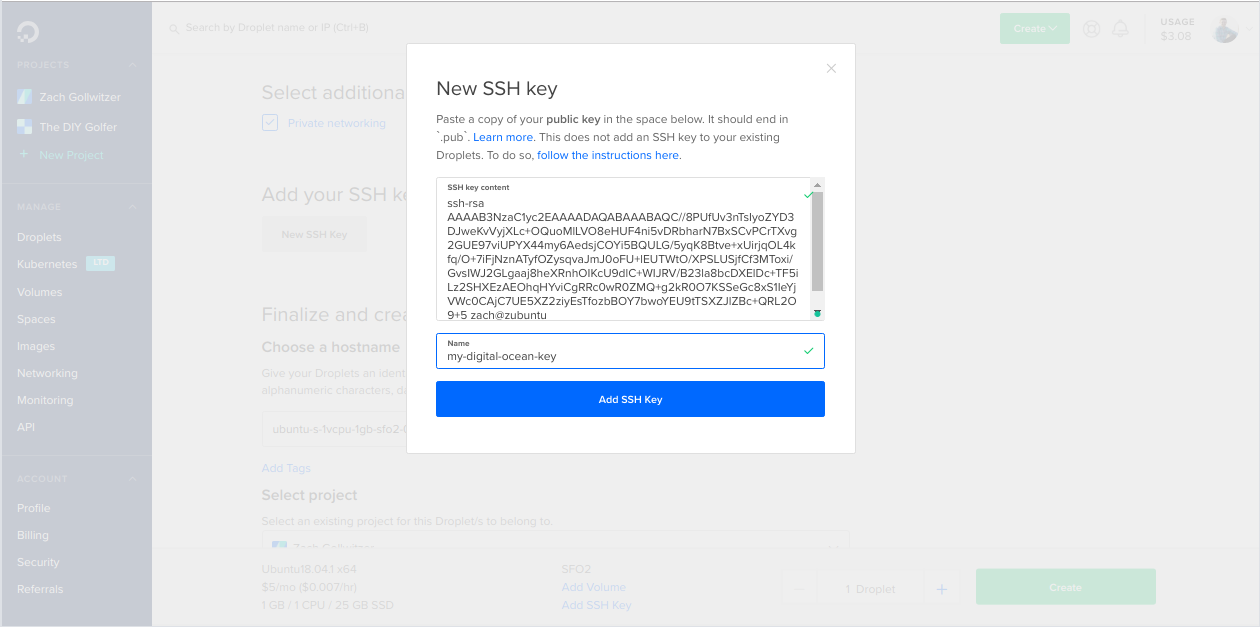
\includegraphics[width=0.9\linewidth]{blog/2019/bash-essentials/digital-ocean-key.png}

  \caption{Регистрация пользователя виртуальной машины на DigitalOcean}
  \label{fig:userreg}
\end{figure}
Как только это сделано, можете создавать свою виртуальную машину. Теперь
надо найти IP-адрес новой виртуальной машины и ввести в терминале
следующую команду.

\begin{minted}{bash}
ssh -p 22 root@157.230.167.2
\end{minted}

Эта команда должна подключить текущий терминал к новому VPS.

\hypertarget{Permanently-Add-Keys-to-ssh-agent}{%
\subsubsection{\texorpdfstring{\protect\hyperlink{Permanently-Add-Keys-to-ssh-agent}{}Добавление
постоянных ключей в
ssh-agent}{Добавление постоянных ключей в ssh-agent}}\label{Permanently-Add-Keys-to-ssh-agent}}

Обычно это не проблема для Linux, но на Mac нужно будет изменить
некоторые настройки по умолчанию. По умолчанию любой ключ, который не
является файлом \texttt{id\_rsa} не будет добавлен ни в программу
ssh-agent, ни в <<связку ключей>> Mac. Каждый раз, когда надо подключиться
к виртуальной машине, нужно будет добавлять ключ ssh. Например, есть
ключ под названием \texttt{digital-ocean}, который используется для
входа цифровые <<капли океана>>.

\begin{minted}{bash}
# Загружает необходимые переменные среды
eval `ssh-agent -s`

# Добавляется ssh key
ssh-add -K ~/.ssh/digital-ocean

# Подключение
ssh -p 22 root@<some-ip-address>
\end{minted}

Чтобы избежать таких повторений при входе в систему Mac нужно будет
изменить \texttt{\textasciitilde{}/.ssh/config} и добавить следующую
запись:

\begin{minted}{bash}
Host *
  UseKeychain yes
  AddKeysToAgent yes
  IdentityFile ~/.ssh/id_rsa
  IdentityFile ~/.ssh/digital-ocean
\end{minted}

Указание поля Host * обозначает возможность подключения к любому
серверу. Символ * можно заменить доменом, например github.com. Кроме
того, настройка сообщает агенту использовать связку ключей, добавлять
ключи и использовать два файла идентификации, перечисленные как <<пароли>>
к удаленным соединениям.

\hypertarget{From-local-computer-to-remote-machine}{%
\subsubsection{\texorpdfstring{\protect\hyperlink{From-local-computer-to-remote-machine}{}С
локального компьютера на
удаленный}{С локального компьютера на удаленный}}\label{From-local-computer-to-remote-machine}}

Далее покажем, как передавать файлы между локальным и удаленным
компьютером. Для этого используется утилита \texttt{scp}.

Например, загрузим \texttt{sample-file.txt} на удаленную машину:

\begin{minted}{bash}
scp -r sample-file.txt root@157.230.167.2:~/
\end{minted}

В результате файл \texttt{sample-file.txt} будет загружен, используя
пользователя \texttt{root}, файл будет помещен в домашний каталог
\texttt{\textasciitilde{}/} на уделенной машине. Можно указать любое
месторасположение размещения файлов на удаленном компьютере. Оно
указывается после \texttt{:}, которое после IP-адреса.

\hypertarget{From-remote-machine-to-local-computer}{%
\subsubsection{\texorpdfstring{\protect\hyperlink{From-remote-machine-to-local-computer}{}С
удаленного компьютера на
локальный}{С удаленного компьютера на локальный}}\label{From-remote-machine-to-local-computer}}

Чтобы загрузить файл с удаленного компьютера на локальный надо запустить
следующую команду.

\begin{minted}{bash}
scp -r root@157.230.167.2:~/sample-file.txt ~/Downloads
\end{minted}

Загруженный файл будет помещен в папку
\texttt{\textasciitilde{}/Downloads} локального компьютера.

\hypertarget{Downloading-packages-to-your-remote-machine-with-wget}{%
\subsubsection{\texorpdfstring{\protect\hyperlink{Downloading-packages-to-your-remote-machine-with-wget}{}Загрузка
пакетов на удаленный компьютер с помощью
wget}{Загрузка пакетов на удаленный компьютер с помощью wget}}\label{Downloading-packages-to-your-remote-machine-with-wget}}

Иногда нужно загрузить пакеты программного обеспечения из Интернета на
VPS. Поскольку нет графического интерфейса, нужно выполнить команду в
командной строке. Допустим, по какой-то причине надо загрузить картинку
Google на VPS.

Вот няшная картинка хаски -
\url{https://cdn.orvis.com/images/DBS_SibHusky.jpg}

Загрузить ее это на наш VPS можно, используя следующую команду.

\begin{minted}{bash}
wget -O my-custom-picture.jpg https://cdn.orvis.com/images/DBS_SibHusky.jpg
\end{minted}

В результате фотография будет загружена и сохранена как
\texttt{my-custom-picture.jpg} в каком-либо каталоге, в котором потом
можно ее можно обрабатывать различными командами и программами.

\hypertarget{Using-VSCode-with-your-remote-machine}{%
\subsubsection{\texorpdfstring{\protect\hyperlink{Using-VSCode-with-your-remote-machine}{}Использование
VSCode через удаленное
соединение}{Использование VSCode через удаленное соединение}}\label{Using-VSCode-with-your-remote-machine}}

Конечно, можно использовать текстовый редактор Vim для решения всех
задач в разработке программ прямо на VPS, но хорошо иметь под рукой
многофункциональный текстовый редактор, такой как VSCode. Редактор
VSCode может использоваться для редактирования файлов на VPS, это
достигается при помощи команды \texttt{rmate}. Для включения этой
функции откройте в VSCode и загрузите расширение (extension) под
названием «Remote VSCode». После загрузки откройте настройки, набрав
ctrl-shift + P и набрав <<\textgreater Preferences:Open User Settings>>.
Пролистайте вниз и найдите раскрывающийся список <<Extensions>> и выберите
<<Remote VSCode>>. Далее требуется добавить следующие настройки:

\begin{minted}{bash}
Remote Host: 127.0.0.1
Remote Port: 52698
Remote Onstartup: True (will be a checkbox)
\end{minted}

Наберите ctrl-shift P и <<\textgreater Remote: Start Server>>. Это
запустит удаленный сервер. Теперь в локальном терминале наберите команду
подключения к VPS.

\begin{minted}{bash}
ssh -R 52698:127.0.0.1:52698 root@157.230.167.2
\end{minted}

Замените IP-адрес своим. Затем установите утилиту \texttt{rmate} на VPS.

\begin{minted}{bash}
sudo wget -O /usr/local/bin/rmate \
  https://raw.github.com/aurora/rmate/master/rmate
sudo chmod a+x /usr/local/bin/rmate
\end{minted}

Редактировать файлы на VPS с помощью VSCode можно, если выполнить
команду в командной строке VPS!

\begin{minted}{bash}
rmate sample-file.txt
\end{minted}

\hypertarget{Networking-on-Command-Line}{%
\subsection{\texorpdfstring{\protect\hyperlink{Networking-on-Command-Line}{}Управление
сетью в командной
строке}{Управление сетью в командной строке}}\label{Networking-on-Command-Line}}

Приобретение навыков управления сетью в командной строке -- это огромная
и интересная задача. По этой теме написано много книг и учебников,
поэтому не будем рассматривать все вопросы. В этом разделе описаны
наиболее распространенные сетевые утилиты Bash, которые можно
использовать для диагностики сетевых проблем на компьютере. Если вы
совершенно не знакомы с концепциями сетей, то некоторый базовый уровень
знаний можно получить читая этот раздел.

\hypertarget{Your-home-network-and-the-internet}{%
\subsubsection{\texorpdfstring{\protect\hyperlink{Your-home-network-and-the-internet}{}Сеть
в доме и доступ в
Интернет}{Сеть в доме и доступ в Интернет}}\label{Your-home-network-and-the-internet}}

Чтобы разобраться в командах, которые далее будут запускаться, нужно
иметь хотя бы базовое понимание сетевых технологий.

\begin{enumerate}
\tightlist
\item
  Беспроводная карта компьютера
\item
  Маршрутизатор
\item
  Модем
\item
  Что такое Интернет-провайдер (ISP)
\item
  Система доменных имен (DNS), серверы имён, регистраторы
\end{enumerate}

Иногда модем и маршрутизатор - это одно и то же, но здесь они разделены
для лучшего понимания темы. К концу раздела \emph{вы получите понимание
на высоком уровне, что происходит, когда вы набираете
\href{http://www.thediygolfer.com}{<<www.thediygolfer.com>>} в браузере}.
Выбран именно этот сайт, потому что он принадлежит Заку (автору
данного руководства). Это позволит понять компоненты, составляющие
технологии. Эти концепции сложно объяснить с помощью сложных веб-сайтов,
таких как \href{http://www.google.com}{www.google.com} потому что их
инфраструктура очень сложна. Эти же концепции применимы независимо от
того, какой веб-сайт вы посещаете, но будем следовать правилу "как можно
проще".

\emph{Примечание: некоторые IP-адреса и адреса серверов изменены на
протяжении всего руководства, чтобы защитить конфиденциальность Зака,
однако указанные изменения не влияют концептуально на излагаемый
материал.}

Начнем с диаграммы, которая демонстрирует процесс поиска веб-сайта (рис.~\ref{fig:pageoading}).

\begin{figure}[tbh]
  \centering
  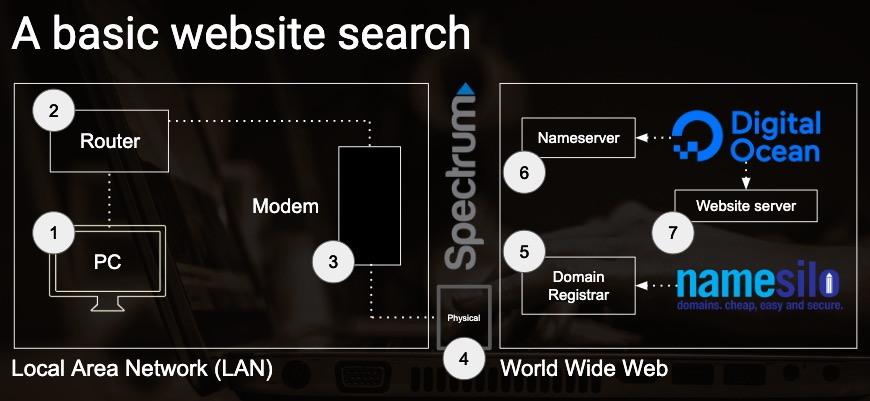
\includegraphics[width=0.9\linewidth]{blog/2019/bash-essentials/basic-web-search.jpg}

  \caption{Процедура загрузки интернет-страницы}
  \label{fig:pageloading}
\end{figure}

Каждый фрагмент технологии пронумерован и иллюстрирует общий поток
информации при выполнении поиска в Интернете. В большинстве случаев все
начинается с шага №1, тут необходимо понимать, что такое
интернет-провайдер (ISP) и какие услуги он предоставляет. Сервисы
интернет-провайдеров во многих случаях сбивают с толку, потому что они
предлагают несколько услуг, здесь будем считать, что интернет-провайдеры
предлагает только доступ Интернет в качестве услуги. Интернет-провайдер
- это компания, которая владеет оборудованием и подключает к этому
оборудованию клиентов, таким образом предоставляя ему интернет-услуги. О
каком оборудовании мы говорим? Многие интернет-провайдеры имеют
оборудование для передачи аналоговых сигналов, известных как «Интернет».

\begin{itemize}
\tightlist
\item
  Коаксиальные кабели, что сейчас уже не встречается
\item
  Кабели неэкранированной витой пары (UTP, 100 МГц)
\item
  Кабели с экранированной витой парой (STP)
\item
  Волоконно-оптические кабели (самый быстрый тип, много оптики лежит на
  дне океана)
\end{itemize}

Технологии предоставляют несколько способов <<доставки>> Интернета в дом,
но наиболее распространенным является провода UTP. Другие варианты
включают подземные кабели и спутниковые тарелки. Передача интернета "по
проводам" часто сбивает людей с толку, потому что, исходя из названия,
можно предположить, что только телефонные сигналы могут передаваться по
телефонным проводам. Но это не наш случай Интернет ранее функционировал
на инфраструктуре телефонной системы, и в настоящее время в каждом
телефонном проводе организовано несколько каналов связи. Это называется
«широкополосным доступом», и по этой причине можно одновременно
разговаривать по телефону, смотреть Netflix и искать информацию в
Интернете. Раньше приходилось использовать «дозвон», когда пользователи
буквально «звонили» по телефонной линии для доступа в Интернет.

Независимо от того, какой метод подключения к Интернету использует
интернет-провайдер, всегда сталкиваемся с одной и той же проблемой.
Сигналы, проходящие по телефонной линии до вашего интернет-провайдера
\emph{аналоговые}, в то время как работа компьютера соответствует
\emph{цифровой} технологии передачи сигналов (единицы и нули). Вот где
используется устройство-модем.

Модем принимает аналоговый сигнал, преобразует его в цифровой и
отправляет на маршрутизатор. Пока нам не важно, что делает
маршрутизатор, но теперь есть начальная информация, необходимая для
понимания диаграммы. Интернет-провайдеры владеют тоннами проводов и
инфраструктурой, к которой подключаются миллионы людей, а также между
провайдерами существуют соединения. Это составляет Интернет, и он
поставляется в дом через телефонные провода, подземные кабели или
спутник. При достижении дома, он преобразуется в цифровые сигналы модемом
и отправляется на маршрутизатор. Теперь наш вопрос: что маршрутизатор
делает с сигналом?

Это сложный вопрос, так как теперь рассмотрим поток информации, начиная
с первого звена в цепи -- компьютера. Подключение к Интернету,
предоставляемое провайдером, бесполезно, если оно не используется,
поэтому сначала нужно сделать интернет-запрос, чтобы увидеть его в
действии. Как уже упоминалось, Для выполнения поиска на главной странице
сайта \href{http://www.thediygolfer.com}{www.thediygolfer.com}

Запускаем компьютер, открываем браузер (в данном случае Google Chrome) и
набираем <<\href{http://www.thediygolfer.com}{www.thediygolfer.com}>> в
строке адреса. Нажимаем ВВОД. Теперь, используя эту информацию,
браузерное приложение "должно отправиться в путешествие по всемирной
паутине", чтобы найти веб-сайт. Веб-сайт -- это набор файлов, находящихся
в серверном приложении, запущенном на каком-то компьютере где-то в мире.
В нашем случае сайт, который мы ищем, находится где-то в Нью-Йорке, но
наш браузер еще этого не знает!

Первый шаг, который предпримет компьютер, - это формирование базового
HTTP-запроса GET. Не важно понимать, что это означает, но нужно
понимать, что это структурированный способ взаимодействия браузера. Вот
этот GET-запрос.

\begin{minted}{bash}
GET / HTTP/1.1
Host: www.thediygolfer.com
Connection: keep-alive
Cache-Control: max-age=0
Upgrade-Insecure-Requests: 1
User-Agent: Mozilla/5.0 (X11; Linux x86_64) AppleWebKit/537.36 ...
Accept: text/html,application/xhtml+xml,application/xml;q=0.9, ...
Accept-Encoding: gzip, deflate, br
Accept-Language: en-US,en;q=0.9
\end{minted}

Не будем разбираться в каждой строке, но можно сделать разумную оценку,
что означает каждая строка. Посмотрим на строку <<Host:
\href{http://www.thediygolfer.com}{www.thediygolfer.com}>>. Эта
информация вместе с остальной помещается в <<packet>>, который затем
отправляется маршрутизатору через соединение между маршрутизатором и
беспроводной картой вашего компьютера. Как только он достигнет
маршрутизатора, устройство будет действовать как «сортировочная машина»
и направлять запрос туда, куда нужно. Настоящий вопрос: как
маршрутизатор узнает, куда должен идти этот запрос?

Здесь на помощь приходит система доменных имен (DNS). По всему миру
тысячи серверов работают для одной цели. Эта цель -- преобразовать
удобочитаемые доменные имена в IP-адреса. Другими словами, маршрутизатор
знает, куда направить запрос, потому что у него есть доступ к серверу
доменных имен. У каждого маршрутизатора есть DNS-сервер по умолчанию,
который он использует. Данный маршрутизатор использует сервер доменных
имен, расположенный по адресу \texttt{208.67.222.123}. Если набрать этот
IP-адрес в поисковый сайт, например
\url{https://whatismyipaddress.com/ip}, можно получить следующий ответ
сервера DNS.

\begin{minted}{bash}
IP:   208.67.222.123
Decimal:    3494108795
Hostname:   resolver1-fs.opendns.com
ASN:  36692
ISP: OpenDNS, LLC
Organization: OpenDNS, LLC
Services: None detected
Type:    Corporate
Assignment:  Static IP
Blacklist:
Continent:    North America
Country: United States us flag
Latitude:    37.751  (37° 45' 3.60'' N)
Longitude:   -97.822  (97° 49' 19.20'' W)
\end{minted}

Сразу видно, что этим сервером управляет OpenDNS LLC, это всем известный
DNS-сервер. Другой хорошо известный DNS-сервер - это Google, работающий
по IP-адресу 8.8.8.8.

\begin{minted}{bash}
IP:   8.8.8.8
Decimal:   134744072
Hostname:    google-public-dns-a.google.com
ASN:    15169
ISP: Google
Organization:   Google
Services:   None detected
Type:    Corporate
Assignment:  Static IP
Blacklist:
Continent:    North America
Country: United States us flag
Latitude:    37.751  (37° 45' 3.60'' N)
Longitude:   -97.822  (97° 49' 19.20'' W)
\end{minted}

Маршрутизатор свяжется со своим DNS-сервером по умолчанию, который затем
выполнит поиск адреса
<<\href{http://www.thediygolfer.com}{www.thediygolfer.com}>>.
Предполагая, что он не найдет его сразу в своем кеше, он начнет искать с
базы данных корневого домена для \texttt{.com}, домена верхнего уровня,
размещенного на хостинге компании VeriSign. Это известно потому что
\href{https://www.iana.org/domains/root/db/com.html}{это можно узнать на
IANA.org}. Корневой базе данных известно, где находится
\texttt{thediygolfer.com} потому, что он зарегистрирован у официального
регистратора
\href{https://www.namesilo.com/register.php?rid=21c9e40dd}{NameSilo}.
При регистрации домена, он был помещен в базу данных домена верхнего
уровня \texttt{.com}, размещенную в Verisign. ??? Затем я сказал
NameSilo, где хочу указать доменное имя. ??? Поскольку сайт размещен на
DigitalOcean, NameSilo было сообщено указывать на
\texttt{thediygolfer.com} его DNS-серверами DigitalOcean, а именно:

\begin{minted}{bash}
173.245.58.51
173.245.59.41
198.41.222.173
\end{minted}

Любой из этих трех серверов знает, какой IP-адрес соответствует
\texttt{thediygolfer.com}. На этом этапе мой маршрутизатор запустил
сервер OpenDNS по умолчанию для поиска\texttt{\ thediygolfer.com}, но не
сумев найти его, OpenDNS перенаправил маршрутизатор в базу данных
корневого домена, который, затем, нашел домен и перешел на серверы имен
Digital Ocean, точно знающие, где находится физический сервер сайта.
Маршрутизатор рассчитает самый быстрый путь до цели и перешлет пакет
запроса в соответствующем направлении.

С другой стороны, сервер, на котором работает веб-сайт, найдет
запрошенный HTML-документ (домашняя страница), упакует его и отправит
обратно на запрашивающий IP-адрес (мой компьютер). Пакеты будут
доставлены на домашний маршрутизатор, но как маршрутизатор узнает, где
находится компьютер? Здесь подходим к локальным сетям.

Маршрутизатор представляет собой «локальную сеть» и фактически имеет
динамический внешний IP-адрес (DHCP), который время от времени меняться
провайдером. Это нормально, потому что отосланный запрос имеет текущий
IP-адрес домашней сети, и поэтому сервер, отправляющий информацию,
найдет эту сеть. Как только он находит сеть, маршрутизатор отвечает за
маршрутизацию информации на нужное устройство в локальной сети.

В доме есть несколько устройств (ноутбук, настольный компьютер, принтер
и т.д.), Поэтому для каждого устройства в домашней сети потребуется свои
IP-адреса. Было бы сложно управлять новым IP-адресом для каждого
устройства в <<дикой природе>>, но с нашей локальной сетью это просто.
Сеть имеет IP-адрес, который называется «шлюзом по умолчанию». Этот
IP-адрес представляет все устройства в сети, через него уходит и входит
трафик Интернет. Внутри локальной сети каждое устройство имеет
уникальный IP-адрес в пределах адресного пространства локальной сети,
заданного соответствующей маской. Эту тему невозможно понять без
усвоения сетевых технологий. Для более глубокого усвоения темы есть
\href{blog/2019/ip-addresses-netmasks}{отдельный пост}, который
предназначен тем, кому интересно. Если вы решите не тратить время на
чтение, вот некоторые заметки и диаграмма (рис.~\ref{fig:netparms}).

\begin{figure}[tbh]
  \centering
  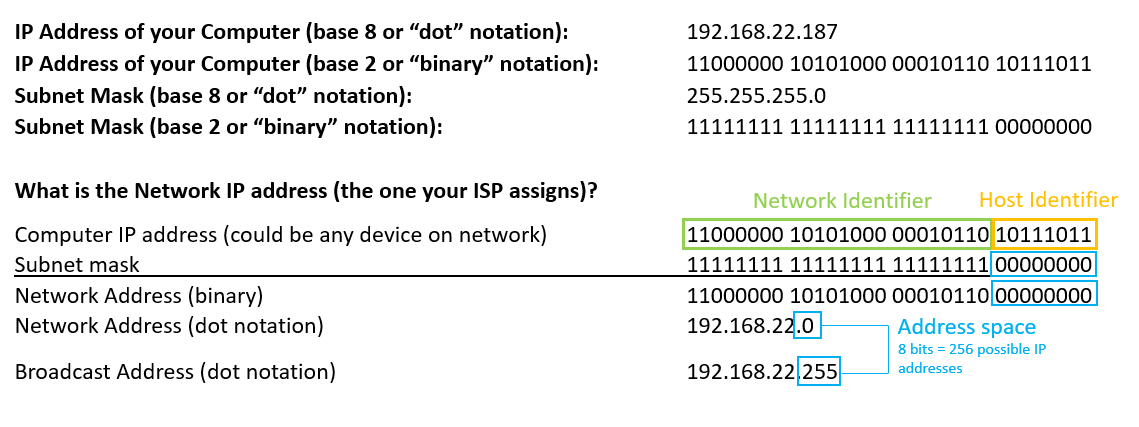
\includegraphics[width=0.9\linewidth]{blog/2019/bash-essentials/ipaddresses.PNG}

  \caption{Вычисление параметров сети}
  \label{fig:netparms}
\end{figure}
\begin{itemize}
\tightlist
\item
  Ваш интернет-провайдер назначает вашей сети IP-адрес и маску подсети.
  Их объединение дает адрес «сети» или «шлюза по умолчанию». Другими
  словами, IP-адрес состоит из двух частей -- идентификатора сети и
  идентификатора «адресного пространства» сети.
\item
  Маски подсети используются для экономии адресного пространства,
  используемого одной сетью. Адресное пространство -- это диапазон
  IP-адресов, доступных для устройств в сети (например, 192.0.168.1,
  192.0.168.2, 192.0.168.3, 192.0.168.4,\ldots, 192.0.168.254)
\item
  DHCP - это сервер (обычно работающий на маршрутизаторе), который
  назначает новому устройству IP-адрес, когда оно входит в сеть. Этот
  IP-адрес всегда будет в адресном пространстве, определенном маской
  подсети.
\end{itemize}

В любом случае вернемся к нашему обсуждению ... У нас есть несколько
пакетов данных, которые приходят с сервера веб-сайта и доставляются на
наш маршрутизатор. Устройство, с которого вы выполняли поиск,
обнаруживается маршрутизатором, данные веб-сайта доставляются, и
домашнюю страницу
\href{http://www.thediygolfer.com}{www.thediygolfer.com} отображается в
браузере. Этот процесс происходит за секунды (или даже миллисекунды).
Обладая этими базовыми знаниями, теперь можно взглянуть на некоторые
команды bash, которые помогут нам диагностировать сетевые проблемы.

\hypertarget{ifconfig}{%
\subsubsection{\texorpdfstring{\protect\hyperlink{ifconfig}{}Утилита
ifconfig}{Утилита ifconfig}}\label{ifconfig}}

Команда ifconfig предоставит нам информацию о домашней локальной сети,
которую мы только что обсудили. Эту команду также можно использовать для
установки новых настроек, но нам достаточно просто посмотреть на
результат. Наберите \texttt{ifconfig} в терминале, в результате
получится результат, похожий на следующий.

\begin{minted}{text}
enp37s0: flags=4099<UP,BROADCAST,MULTICAST>  mtu 1500
        ether 70:85:c2:7c:ff:f2  txqueuelen 1000  (Ethernet)
        RX packets 0  bytes 0 (0.0 B)
        RX errors 0  dropped 0  overruns 0  frame 0
        TX packets 0  bytes 0 (0.0 B)
        TX errors 0  dropped 0 overruns 0  carrier 0  collisions 0

enx000f00de66da: flags=4163<UP,BROADCAST,RUNNING,MULTICAST>  mtu 1500
        inet <hidden for privacy>  netmask 255.255.255.0  broadcast ...
        inet6 <hidden for privacy>  prefixlen 64  scopeid 0x20<link>
        ether 00:0f:00:de:66:da  txqueuelen 1000  (Ethernet)
        RX packets 265073  bytes 821138812 (821.1 MB)
        RX errors 0  dropped 1451  overruns 0  frame 0
        TX packets 44132  bytes 102041651 (102.0 MB)
        TX errors 0  dropped 2100 overruns 0  carrier 0  collisions 0

lo: flags=73<UP,LOOPBACK,RUNNING>  mtu 65536
        inet 127.0.0.1  netmask 255.0.0.0
        inet6 ::1  prefixlen 128  scopeid 0x10<host>
        loop  txqueuelen 1000  (Local Loopback)
        RX packets 752935  bytes 54372769 (54.3 MB)
        RX errors 0  dropped 0  overruns 0  frame 0
        TX packets 752935  bytes 54372769 (54.3 MB)
        TX errors 0  dropped 0 overruns 0  carrier 0  collisions 0
\end{minted}

В данной конфигурации есть три записи. Нижняя запись, относящаяся к
интерфейсу «lo», представляет собой конфигурацию интерфейса обратной
связи, его адрес 127.0.0.1, localhost, он обычно используется для
разработки веб-приложений. Первая запись «enp37s0» кажется пустой
конфигурацией. Средняя запись «enx000f00de66da» отображает IP-адрес
устройства, подключенного к маршрутизатору (локальной сети), маску
подсети и широковещательный адрес этой сети.

Вот где понимание IP-адресов и
подсетей в локальной сети полезно, потому что указанный адрес INET на
самом деле не является общедоступным IP-адресом, распознаваемым
маршрутизаторами Интернета. Этот IP-адрес является \emph{локальным},
который нужно преобразовать во <<внешний>> IP-адрес сети, объединив его с
маской подсети. Также указан широковещательный адрес, но он легко
получается его из IP-адреса и маски подсети.

Если я наберу ifconfig на другом компьютере в своей сети,
широковещательный адрес и маска подсети не изменятся, но IP-адрес
изменится. Также есть данные, такие как максимальный размер пакета (MTU)
и счетчики пакетов RX/TX, которые указывают, сколько пакетов было
передано в локальную сеть и из нее. Эти значения постоянно
увеличиваться.

\hypertarget{ping}{%
\subsubsection{\texorpdfstring{\protect\hyperlink{ping}{}Программа
ping}{Программа ping}}\label{ping}}

Программа \texttt{ping} - это базовая утилита, используемая для проверки
связи между устройствами в локальной сети или даже между устройствами за
пределами локальной сети. Команда полезна в случаях отсутствия браузера
для проверки подключения к Интернету. У команды есть различные флаги, но
единственное, что вам нужно знать сейчас, - это флаг \texttt{-c},
позволяющий указывать количество пакетов, которые мы хотим отправить
серверу.

\begin{minted}{bash}
ping -c 5 thediygolfer.com
\end{minted}

\begin{minted}{bash}
PING thediygolfer.com (104.248.115.234) 56(84) bytes of data.
64 bytes from 104.248.115.234 (104.248.115.234): icmp_seq=1 ttl=48 time=36.0 ms
64 bytes from 104.248.115.234 (104.248.115.234): icmp_seq=2 ttl=48 time=49.9 ms
64 bytes from 104.248.115.234 (104.248.115.234): icmp_seq=3 ttl=48 time=35.2 ms
64 bytes from 104.248.115.234 (104.248.115.234): icmp_seq=4 ttl=48 time=34.4 ms
64 bytes from 104.248.115.234 (104.248.115.234): icmp_seq=5 ttl=48 time=35.3 ms

--- thediygolfer.com ping statistics ---
5 packets transmitted, 5 received, 0% packet loss, time 4005ms
rtt min/avg/max/mdev = 34.427/38.183/49.912/5.885 ms
\end{minted}

Приведенная выше команда отправляет на главную страницу сайта 5
отдельных запросов, в результате получаем данные о каждом запросе.
Основываясь на этих данных, получается, что наш компьютер подключен к
сети и может подключиться к thediygolfer.com.

\hypertarget{traceroute}{%
\subsubsection{\texorpdfstring{\protect\hyperlink{traceroute}{}Программа
traceroute}{Программа traceroute}}\label{traceroute}}

Команда traceroute - отличный способ понять, как компьютер находит
сервер и через какие маршрутизаторы проходит запрос на
\href{http://www.thediygolfer.com}{www.thediygolfer.com}. Как было
упомянуто ранее сервер сайта находится где-то в Нью-Йорке, и команда
traceroute подтверждает это, показывая путь, по которому пакеты
добираемся туда.

Эта команда может не быть установлена на компьютере по умолчанию, в этом
случае ее нужно установить.

\begin{minted}{bash}
# Linux
sudo apt-get update && sudo apt install inetutils-traceroute
\end{minted}

На Mac доступ к функциям traceroute осуществляется при помощи Network
Utility. При запуске traceroute, получаем следующий результат.

\begin{minted}{bash}
traceroute --resolve-hostnames -q 1 -w 5 -I thediygolfer.com
\end{minted}

\begin{minted}{bash}
traceroute to thediygolfer.com (104.248.115.234), 64 hops max
  1   192.168.0.1 (_gateway)  53.296ms
  2   142.254.145.21 (142.254.145.21)  10.502ms
  3   24.164.117.37 (24.164.117.37)  15.953ms
  4   65.189.128.164 (65.189.128.164)  11.035ms
  5   65.29.1.87 (be14.pltsohae01r.midwest.rr.com)  18.102ms
  6   65.29.1.28 (be25.clmkohpe01r.midwest.rr.com)  23.729ms
  7   66.109.6.68 (bu-ether15.chctilwc00w-bcr00.tbone.rr.com)  31.967ms
  8   66.109.5.136 (66.109.5.136)  34.155ms
  9   66.109.5.225 (66.109.5.225)  26.993ms
 10   64.86.79.97 (ix-ae-27-0.tcore2.ct8-chicago.as6453.net)  25.094ms
 11   64.86.79.2 (if-ae-22-2.tcore1.ct8-chicago.as6453.net)  33.455ms
 12   216.6.81.28 (if-ae-26-2.tcore2.nto-new-york.as6453.net)  35.629ms
 13   66.110.96.5 (if-ae-12-2.tcore1.n75-new-york.as6453.net)  33.047ms
 14   66.110.96.26 (66.110.96.26)  34.565ms
 15   *
 16   *
 17   104.248.115.234 (104.248.115.234)  35.916ms
\end{minted}

В приведенной выше команде утилите traceroute указано, что необходимо
преобразовать IP-адреса в их имена хостов
(\texttt{-\/-resolve-hostnames}), отправлять только один пакет на
очередной маршрутизатор на пути следования пакета (\texttt{-q\ 1}),
установить тайм-аут для каждого запроса в 5 секунд (\texttt{-w\ 5}) и,
наконец, использовать протокол ICMP вместо UDP (\texttt{-I}). Как
видите, путь начинается со шлюза компьютера, переходит на сервер
Spectrum в Канзасе, подключается к серверу в Чикаго, подключается к
серверам Digital Ocean в Нью-Йорке и, наконец, попадает на сервер
веб-сайта в Нью-Джерси. Показанные места известны, так как ранее они
были найдены автором на
\href{https://whatismyipaddress.com/ip-lookup}{этом онлайн-сервисе}.

\hypertarget{netstat}{%
\subsubsection{\texorpdfstring{\protect\hyperlink{netstat}{}Программа
netstat}{Программа netstat}}\label{netstat}}

Эта команда предоставляет информацию о различных сетевых протоколах
(TCP/IP, UDP, ICMP и т.д.), используемые компьютером. Большая часть
того, что эта программа выводит, выходит за рамки обсуждаемого выше, она
заслуживает упоминания, так как это важный инструмент для понимания
того, как компьютер общается с внешним миром. Например, можно ввести
следующую команду, показывающую, что происходит в различных сетевых
протоколах.

\begin{minted}{bash}
netstat -s
\end{minted}

Результат запуска показан ниже. Обратите внимание, что вывод также
обрезан для краткости, и включены только протоколы IP, TCP и UDP.

\begin{minted}{bash}
Ip:
    400933 total packets received
    0 forwarded
    0 incoming packets discarded
    400933 incoming packets delivered
    296285 requests sent out
    3 outgoing packets dropped
Tcp:
    32175 active connections openings
    28 passive connection openings
    0 failed connection attempts
    4 connection resets received
    1 connections established
    400885 segments received
    300195 segments send out
    41 segments retransmited
    0 bad segments received.
    7 resets sent
Udp:
    28 packets received
    0 packets to unknown port received.
    0 packet receive errors
    43 packets sent
\end{minted}

Еще одно полезное приложение утилиты netstat - узнать, какие порты
используют (<<окрыли>>) процессы на компьютере. Процессы пока не
обсуждались, это на будущее.

\begin{minted}{bash}
netstat -tp
\end{minted}

\begin{minted}{bash}
(Не все процессы могут быть идентифицированы, информация о процессах,
не принадлежащих текущему пользователю не будут отображаться,
нужно быть root-ом, чтобы увидеть их все.)
Активные интернет-соединения (без серверов)
Proto Recv-Q Send-Q Local Address           Foreign Address
   State       PID/Program name
tcp        0      0 zubuntu:35098           stackoverflow.com:https
   ESTABLISHED 26679/chrome --type
\end{minted}

Большая часть вывода этой команды удалена, но здесь видно, что в системе
открыто окно Google Chrome (с идентификатором процесса 26679), и одна из
вкладок открыта на stackoverflow.com. Локальный адрес означает, что
локальный компьютер (zubuntu - полное имя для 127.0.0.1) открыл порт
(сокет) с идентификатором 35098 для данной вкладки в окне Google Chrome.
У каждой вкладки свой сокет.

\hypertarget{dig-host-whois}{%
\subsubsection{\texorpdfstring{\protect\hyperlink{dig-host-whois}{}Программы
dig/host/whois}{Программы dig/host/whois}}\label{dig-host-whois}}

Программы \texttt{dig}, \texttt{host} и \texttt{whois} помогают узнавать
информацию о доменных именах, IP-адресах и механизмах отображения одних
в другие. Как правило, программы \texttt{dig} и \texttt{host}
устанавливаются на компьютер по умолчанию, а вот команду \texttt{whois},
вероятно, придется установить самостоятельно. В Linux она
устанавливается путем выполнения \texttt{sudo\ apt-get\ install\ whois}
в терминале.

Начнем с программы \texttt{dig}, которая помогает запрашивать записи DNS
для IP-адресов (с использованием обратного поиска) или доменного имени.
Используя эту утилиту, можно запросить знакомый нам сайт.

\begin{minted}{bash}
dig thediygolfer.com
\end{minted}

\begin{minted}{bash}
; <<>> DiG 9.9.5-3ubuntu0.15-Ubuntu <<>> thediygolfer.com
;; global options: +cmd
;; Got answer:
;; ->>HEADER<<- opcode: QUERY, status: NOERROR, id: 51716
;; flags: qr rd ra; QUERY: 1, ANSWER: 1, AUTHORITY: 0, ADDITIONAL: 1

;; OPT PSEUDOSECTION:
; EDNS: version: 0, flags:; udp: 4096
;; QUESTION SECTION:
;thediygolfer.com.              IN      A

;; ANSWER SECTION:
thediygolfer.com.       600     IN      A       104.248.115.234

;; Query time: 0 msec
;; SERVER: 172.17.0.1#53(172.17.0.1)
;; WHEN: Wed Feb 27 18:41:22 UTC 2019
;; MSG SIZE  rcvd: 61
\end{minted}

Обратите внимание, что здесь много информации, и по большей части это
комментарии (обозначены ;;). Чтобы сократить результат, можно добавить
флаги \texttt{+noall} и \texttt{+answer}, т.е. показывать только раздел
ответов.

\begin{minted}{bash}
dig thediygolfer.com +noall +answer
\end{minted}

\begin{minted}{bash}
; <<>> DiG 9.9.5-3ubuntu0.15-Ubuntu <<>> thediygolfer.com +noall +answer
;; global options: +cmd
thediygolfer.com.       600     IN      A       104.248.115.234
\end{minted}

В результате просто будет напечатана запись A для сайта в коротком
формате. Можно также запустить \texttt{dig\ thediygolfer.com\ +short},
при этом будет получен аналогичный результат. Но что, если нужны все
записи DNS для домена? Для этого можно добавить опцию \texttt{ANY}.

\begin{minted}{bash}
dig thediygolfer.com ANY +noall +answer
\end{minted}

\begin{minted}{bash}
; <<>> DiG 9.9.5-3ubuntu0.15-Ubuntu <<>> thediygolfer.com ANY +noall +answer
;; global options: +cmd
thediygolfer.com.       3599    IN      A       104.248.115.234
thediygolfer.com.       1799    IN      NS      ns1.digitalocean.com.
thediygolfer.com.       1799    IN      NS      ns2.digitalocean.com.
thediygolfer.com.       1799    IN      NS      ns3.digitalocean.com.
thediygolfer.com.       1799    IN      SOA     ns1.digitalocean.com. \
      hostmaster.thediygolfer.com. 1545305910 10800 3600 604800 1800
\end{minted}

В ответе видно, что домен содержит одну запись A (сопоставление
IP-адреса и имени домена), три записи сервера имен и одна запись «Start
of authority» (SOA), указывающая, что Digital Ocean является
авторитетным источником для записи DNS.

Введем следующую команду, найдем IP-адрес домена.

\begin{minted}{bash}
host thediygolfer.com

# thediygolfer.com has address 104.248.115.234
\end{minted}

Если использовать команду с серверами Google, можно получить больше
записей, так как в их сети размещено много серверов, в том числе,
поддерживающих электронную почту.

\begin{minted}{bash}
host google.com
\end{minted}

\begin{minted}{bash}
google.com has address 108.177.112.139
google.com has address 108.177.112.101
google.com has address 108.177.112.102
google.com has address 108.177.112.100
google.com has address 108.177.112.113
google.com has address 108.177.112.138
google.com has IPv6 address 2607:f8b0:4001:c12::64
google.com mail is handled by 30 alt2.aspmx.l.google.com.
google.com mail is handled by 50 alt4.aspmx.l.google.com.
google.com mail is handled by 40 alt3.aspmx.l.google.com.
google.com mail is handled by 10 aspmx.l.google.com.
google.com mail is handled by 20 alt1.aspmx.l.google.com.
\end{minted}

Наконец, команда \texttt{whois} дает дополнительную информацию о данном
доменном имени или IP-адресе. Она наверняка не установлена по умолчанию,
поэтому выполнив \texttt{sudo\ apt-get\ install\ whois}, можно
установить ее. Вот пример того, как она работает.

\begin{minted}{bash}
whois thediygolfer
\end{minted}

\begin{minted}{bash}
Domain Name: THEDIYGOLFER.COM
Registry Domain ID: 1896554473_DOMAIN_COM-VRSN
Registrar WHOIS Server: whois.namesilo.com
Registrar URL: http://www.namesilo.com
Updated Date: 2018-12-15T15:30:57Z
Creation Date: 2015-01-18T02:22:03Z
Registry Expiry Date: 2020-01-18T02:22:03Z
Registrar: NameSilo, LLC
Registrar IANA ID: 1479
Registrar Abuse Contact Email: abuse@namesilo.com
Registrar Abuse Contact Phone: +1.4805240066
Domain Status: clientTransferProhibited \
  https://icann.org/epp#clientTransferProhibited
Name Server: NS1.DIGITALOCEAN.COM
Name Server: NS2.DIGITALOCEAN.COM
Name Server: NS3.DIGITALOCEAN.COM
DNSSEC: unsigned
URL of the ICANN Whois Inaccuracy Complaint \
  Form: https://www.icann.org/wicf/
\end{minted}

Получена информация о заданном доменном имени.

Существуют и другие инструменты bash, например, \texttt{nslookup},
\texttt{route} и т.д., но которые были рассмотрены, удовлетворят
большинству потребностей пользователей. Если вы не собираетесь быть
администратором, настраивающим сети каждый божий день, вам никогда не
понадобится использовать эти инструменты для редактирования настроек. Но
эти команды также полезны для получения информации о вашей сети и о
внешних сетях.

\hypertarget{Process-Management-and-System-Management}{%
\subsection{\texorpdfstring{\protect\hyperlink{Process-Management-and-System-Management}{}Управление
процессами и
системой}{Управление процессами и системой}}\label{Process-Management-and-System-Management}}

Управление процессами и системой звучит как-то пугающе. Для обычного
пользователя bash существует несколько полезных команд и программ,
которые надо изучить, чтобы получить целостное представление о том, как
работает компьютер.

\begin{itemize}
\tightlist
\item
  Что такое процесс?
\item
  Как создается процесс?
\item
  Как управлять процессами с помощью команд kill, bg и fg
\item
  Как управлять процессами и контролировать системные ресурсы с помощью
  команды top
\end{itemize}

\hypertarget{What-is-a-Process}{%
\subsubsection{\texorpdfstring{\protect\hyperlink{What-is-a-Process}{}Что
такое процесс?}{Что такое процесс?}}\label{What-is-a-Process}}

Если не вдаваться в технические подробности, процесс - это что-нибудь на
исполняющееся на компьютере, который принадлежит пользователю и
потребляет три вида ресурсов системы.

\begin{enumerate}
\tightlist
\item
  Вычислительные (CPU)
\item
  Оперативная память (RAM)
\item
  Периферийные устройства ввода/вывода (input/output,IO)
\end{enumerate}

После загрузки компьютера ядро операционной системы функционирует
постоянно. Ядро постоянно отслеживает состояние всех процессов на
компьютере и выделяет им периодически те или иные системные ресурсы
Процессы конкурируют за системные ресурсы, вытесняя друг друга. Верьте
или нет, при запуске программы, например, Google Chrome, ядро даст ему
ресурсы в течение нескольких микросекунд, а затем произойдет
<<переключение контекстов>>, и эти же ресурсы будут на время отданы
другому процессу. Если Google Chrome захватит 100\% ресурсов во все
100\% времени, компьютер, вероятно, выкинет Google из памяти компьютера
потому, что в ядре есть разные функции поддерживающие функционирование
операционной системы.

\hypertarget{Processes-Behind-the-Scenes}{%
\subsubsection{\texorpdfstring{\protect\hyperlink{Processes-Behind-the-Scenes}{}Закулисы
процессов}{Закулисы процессов}}\label{Processes-Behind-the-Scenes}}

Можно перечислять все возможные команды, но в этом нет особого смысла,
если не понимать последовательность функций, которые выполняет bash и
ядро операционной системы при создании нового процесса. Когда компьютер
запускается, ядро запускает процесс под названием <<init>>, который в
UNIX-системах обычно называется также \texttt{init}, расположенный в
\texttt{/sbin/init}. В современных дистрибутивах этот скрипт находится в
пакете \href{https://en.wikipedia.org/wiki/Systemd}{systemd}. Как только
вы изучите процедуру загрузки системы, вы поймете, что происходит за
кулисами на компьютере. Каждый процесс может начать другой процесс
(обычно терминал начинает новый процесс в результате введенной команды),
сначала создавая свою копию, а затем выполняя новую команду в адресном
пространстве скопированного процесса. Вот иллюстрация, поясняющая
вышесказанное (рис.~\ref{fig:proclc}).

\begin{figure}[tbh]
  \centering

  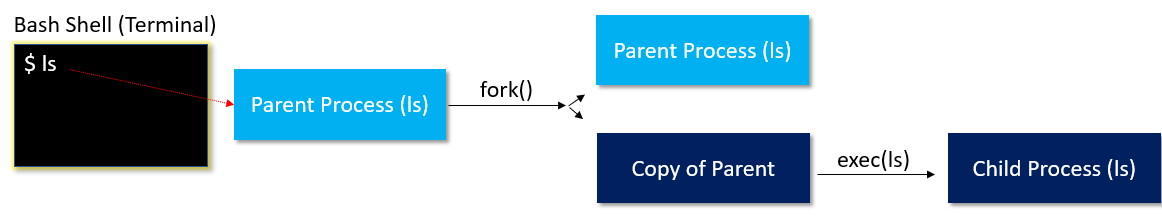
\includegraphics[width=\linewidth]{blog/2019/bash-essentials/processes-linux.png}
%\vspace{-4em}
  \caption{Жизненный цикл процесса}
  \label{fig:proclc}
\end{figure}
Можно отследить этот процесс в терминале самостоятельно, используя
\texttt{strace()} команду. Обратите внимание -- эта команда доступна
только на Linux. Эквивалентная команда на Mac -- \texttt{dtruss}, но она
работает по-другому.

\begin{minted}{bash}
strace ls
\end{minted}

Эта команда позволяет увидеть все системные вызовы, которые были
выполнены при запуске \texttt{ls}. Команда \texttt{ls} на самом деле --
это просто еще один процесс операционной системы. Результат работы
\texttt{strace\ ls}, представленный ниже, обработан, так, чтобы обращать
внимание читателя на наиболее важные части.

\begin{minted}{bash}
execve("/bin/ls", ["ls"], [/* 69 vars */]) = 0

.... пропущено для краткости ....

write(1, "_config.yml  awk-example.sh  db."..., 107_config.yml  \
awk-example.sh  db.json      node_modules    package.json  scaffolds  \
test-permission  yarn.lock
) = 107
write(1, "aapl.csv     data-file.txt   lar"..., 91aapl.csv \
   data-file.txt   large-data.csv  package-lock.json public \
   source    themes
) = 91
close(1)                                = 0
munmap(0x7f1578100000, 4096)            = 0
close(2)                                = 0
exit_group(0)                           = ?
+++ завершается с кодом 0 +++
\end{minted}

Если вам действительно интересно узнать о каждом из системных вызовов в
выводе команды \texttt{strace},
\href{https://stackoverflow.com/a/6334557}{вот отличный пост на
StackOverflow}. Программисты на языке C, вероятно, знакомы с некоторыми
из этих команд.

В приведенном тексте показано, сто команда \texttt{execve}запускает
процесс. Фактически, это fork и exec одновременно. Далее можно будет
посмотреть, как разделять файлы и каталоги. Файлы представляют собой
результат выполнения команды \texttt{ls} в текущем каталоге моей машины.

В конце концов, вывод не важен пользователю bash, но важен для понимания
процедуры запуска и заверения процессы. Важнее уметь \emph{управлять}
процессами. Здесь есть несколько команд, позволяющих ??? позаботится
практически обо всем, что нам когда-либо понадобится в отношении
процессов.

\hypertarget{Foreground-vs-Background-Processes}{%
\subsubsection{\texorpdfstring{\protect\hyperlink{Foreground-vs-Background-Processes}{}Процессы
переднего плана и фоновые
процессы}{Процессы переднего плана и фоновые процессы}}\label{Foreground-vs-Background-Processes}}

Одной из наиболее важных концепций, которую нужно понимать в отношении
процессов, является фоновый режим процесса и <<передний план>> и как
переключаться между ними. После запуска процесса в оболочке bash и пока
процесс исполняется, доступа к терминалу не будет. Если надо остановить
процесс используйте комбинацию клавиш CTRL-C. Есть процессы, которые
выполняются всегда, и где они работают? Почему они не мешают работать в
терминале? Причина в том, что они являются \emph{фоновыми процессами.}
Можем перевести процесс в фоновый режим одним из двух способов:

\begin{enumerate}
\tightlist
\item
  Отправить его в фоновый режим в момент запуска
\item
  Остановить его и отправить в фоновый режим и дать команду продолжения
  исполнения
\end{enumerate}

Первый способ прост. Процесс будет запущен в фоновом режиме если
добавить \texttt{\&} в конце команды. Например, можно запустить команду
\texttt{sleep}, которая будет 20 секунд простаивать в фоновом режиме.

\begin{minted}{bash}
sleep 20 &
\end{minted}

Второй метод немного сложнее и требует от понимания концепции
\emph{сигналов, передаваемых процессам}. Посылка сигналов процессам
осуществляется командой \texttt{kill}. Перечень всех сигналов выводится
в результате команды \texttt{kill\ -l}. Вот наиболее распространенные
сигналы, часто отправляемые в процесс:

\begin{itemize}
\tightlist
\item
  SIGTERM - \texttt{kill} (мягкий сигнал завершения процесса)
\item
  SIGKILL - \texttt{kill\ -9} or \texttt{kill\ -s\ SIGKILL} (силовой
  метод остановки процесса)
\item
  SIGSTOP - \texttt{kill\ -19} or \texttt{kill\ -s\ SIGSTOP}
  ({[}при{]}остановка выполнения процесса)
\item
  SIGCONT - \texttt{kill\ -18} or \texttt{kill\ -s\ SIGCONT} (продолжить
  выполнение процесса)
\item
  SIGINT (CTRL-C) - \texttt{kill\ -2} or \texttt{kill\ -s\ SIGINT}
  (Прервать выполнение процесса)
\item
  SIGTSTP (CTRL-Z) - \texttt{kill\ -20} or \texttt{kill\ -s\ SIGTSTP}
  ({[}при{]}остановка выполняющегося процесса)
\end{itemize}

В нашем примере отправим сигнал SIGTSTP запущенному процессу, чтобы он
перешел в фоновый режим и остановился. Для этого нам понадобится
идентификатор процесса. Чтобы получить этот идентификатор, надо
запустить команду \texttt{ps} (подробнее об этом позже). В данном случае
используем \texttt{google-chrome} с нашим окном браузера, в качестве
примера процесса. Идентификатор процесса - 21124, полученный в
результате выполнения команды \texttt{ps\ a}.

\begin{minted}{bash}
  PID TTY      STAT   TIME COMMAND
 1201 tty7     Ssl+   1:48 /usr/lib/xorg/Xorg -core :0 -seat seat0
     -auth /var/run/lightdm/root/:0 -nolis
 1204 tty1     Ss+    0:00 /sbin/agetty -o -p -- \u --noclear tty1 linux
17824 pts/0    Ss     0:00 -bash
18747 pts/1    Ss+    0:00 /bin/bash
19664 pts/2    Ss+    0:00 -bash

# Вот процесс Google Chrome (этот комментарий был вручную добавлен в
# текст ответа команды ps)
21124 pts/2    SLl    0:03 /opt/google/chrome/chrome

21129 pts/2    S      0:00 cat
21130 pts/2    S      0:00 cat
21133 pts/2    S      0:00 /opt/google/chrome/chrome --type=zygote
 --enable-crash-reporter=2475ab0f-df4d
21134 pts/2    S      0:00 /opt/google/chrome/nacl_helper
21137 pts/2    S      0:00 /opt/google/chrome/chrome --type=zygote
 --enable-crash-reporter=2475ab0f-df4d
21164 pts/2    Sl     0:00 /opt/google/chrome/chrome --type=gpu-proces
s --field-trial-handle=39017447716
21169 pts/2    SLl    0:00 /opt/google/chrome/chrome --type=utility
 --field-trial-handle=390174477165224
21309 pts/2    Sl     0:00 /opt/google/chrome/chrome --type=renderer
 --field-trial-handle=39017447716522
21360 pts/2    Sl     0:01 /opt/google/chrome/chrome --type=renderer
 --field-trial-handle=39017447716522
21398 pts/2    Sl     0:00 /opt/google/chrome/chrome --type=renderer
 --field-trial-handle=39017447716522
21417 pts/2    Sl     0:00 /opt/google/chrome/chrome --type=renderer
 --field-trial-handle=39017447716522
21711 pts/2    Sl     0:01 /opt/google/chrome/chrome --type=renderer
 --field-trial-handle=39017447716522
21751 pts/2    Sl     0:00 /opt/google/chrome/chrome --type=renderer
 --field-trial-handle=39017447716522
21852 pts/2    Sl     0:00 /opt/google/chrome/chrome --type=renderer
 --field-trial-handle=39017447716522
21870 pts/0    R+     0:00 ps a
\end{minted}

На самом деле есть несколько вариантов остановить выполняющийся процесс
Google Chrome. Можно послать сигнал \texttt{SIGTSTP} (т.е. CTRL-Z) или
сигнал \texttt{SIGSTOP} процессу. Любой из них остановит запущенный
процесс и вернет нам доступ к терминалу. Отправим процессу сигнал
\texttt{SIGSTOP} из другого терминального окна.

\begin{minted}{bash}
kill -s SIGSTOP 21124
# `kill -19 21124` также работает
\end{minted}

Заметим, когда вы пытаетесь сделать что-либо в окне Chrome, он не
работает, потому что он -- приостановленный процесс. Теперь можно снова
запустить процесс, но на этот раз запустим его в фоновом режиме. Для
этого перейдите в терминал, на котором находится остановленный Google
Chrome, и введите команду \texttt{jobs}. В результате получите список
заданий для данного терминала. Найдем номер, по которому идентифицируем
Google Chrome (в данном случае -- задание №1), выполним команду.

\begin{minted}{bash}
bg %1
\end{minted}

Google Chrome теперь перезапущен и работает в фоновом режиме. Снова
остановим его и вернем на передний план.

\begin{minted}{bash}
# Останавливает процесс
kill -s SIGSTOP 211124

# Запускает процесс
kill -s SIGCONT 211124

# Перевод процесса в фоновый режим
fg %1
\end{minted}

\hypertarget{ps-and-top-commands-system-performance-management}{%
\subsubsection{\texorpdfstring{\protect\hyperlink{ps-and-top-commands-system-performance-management}{}Команды
ps и top (управление общей производительностью
системы)}{Команды ps и top (управление общей производительностью системы)}}\label{ps-and-top-commands-system-performance-management}}

Есть две команды, показывающие процессы, выполняемые в настоящее время
на нашем компьютере. В 99\% случаев эти команды взаимозаменяемы. Разница
между командами заключается в уровне интерактивности, опыт показывает,
что используются они часто и обе. Например, при запуске \texttt{top}
получаем список процессов. Этот список не просто выдается, но и
отслеживает статус каждого процесса в реальном времени. Поскольку top
интерактивен, другие сценарии не могут использовать его для получения
информации о процессах без специальных настроек (т.е. с использованием
«пакетного» режима). Вот где пригодится команда \texttt{ps}. Команда
используется внутри скриптов bash для получения необходимой информации.
Поскольку мы не собираемся разрабатывать сложные скрипты использования
процессов, первую очередь упор сделаем на \texttt{top}, поскольку она
является более удобной для пользователя. Можно изучить страницы
руководства man для команды \texttt{ps}, где перечисляются эквивалентные
команды тем, о которых далее идет речь, например, \texttt{ps\ ax}
распечатывает все ваши текущие процессы.

Приоритетом в изучении здесь является интерфейс команды \texttt{top} и
что нужно искать на экране. Программа top - это не просто команда bash,
она имеет свои собственные обширные возможности. Обычные пользователи
bash не используют большинство этих возможностей, приведем самые
полезные (рис.~\ref{fig:topscreen}).

\begin{figure}[tbh]
  \centering
  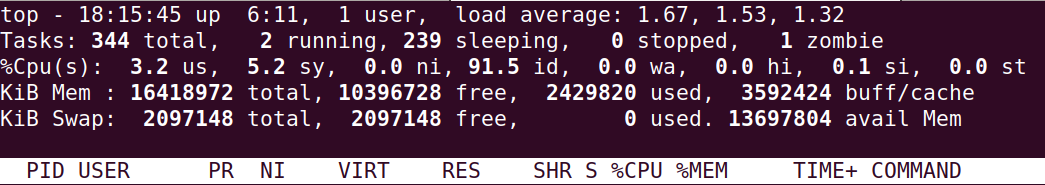
\includegraphics[width=0.9\linewidth]{blog/2019/bash-essentials/top-header.png}

  \caption{Экран команды top}
  \label{fig:topscreen}
\end{figure}
При первом запуске программы top, экран заполнится информацией, как на
рисунке. Экран включает пять строк, начиная с верхней строки (1) и
заканчивая нижней строкой (5), разберем, какую информацию они
отображают.

\begin{enumerate}
\tightlist
\item
  Общая информация
\item
  Показывает различные типы задач, выполняемые на компьютере. Задачи
  могут находиться в состоянии running (выполняется), stopped
  (остановлен), sleeping (простой) или zombie (зомби). Суть их
  интуитивно понятна, за исключением процессов в состоянии зомби. Такие
  процессы является всего лишь процессами, которые погибают, но все еще
  перечислены в таблице процессов, как правило, потому, что родительский
  процесс не смог вычистить его ресурсы.
\item
  Статистика времени использования процессора, включая us (время
  пользователя, un-niced), sy (время системы), ni (время пользователя,
  niced), id (время холостого хода), и wa (время ожидания В-В). Столбцы
  hi, si, и st нам не важны. Можно вычислить общее время пользователя
  (время, необходимое для запуска непосредственно кода программы) -
  сумма us и ni. Данные этой строки будут полезны когда будем
  отфильтровать процессы.
\item
  Cстатистика использования оперативной памяти. В режиме отображения всех
  процессов при недостатке свободная памяти может отображаться красный
  флаг, сигнализирующий, что память заканчивается.
\item
  Статистика памяти swap (подкачки). Подкачка используется только тогда,
  когда реальная память исчерпана, так низкие цифры в <<свободной>> части
  \emph{реальной памяти} и высокие цифры в <<использованной>> части
  \emph{своп} - признак возникновения проблемы производительности
  системы, что, как правило, вызвано слишком малым размером оперативной
  памяти.
\end{enumerate}

Наблюдая за текстом, выдаваемом командой top, можно заметить, что он
обновляется каждые несколько секунд. Таким образом, мы получаем информацию
о состоянии компьютера в реальном времени. Интервалом обновления также
можно управлять. Интервал настраивается двумя способами - «статическим»
и «интерактивным». В статическом режиме конфигурация программы top
устанавливается в командной строке. Например, можно запустить программу
top так:

\begin{minted}{bash}
top -d 10
\end{minted}

При этом в top будет установлен интервал 10 секунд. Значение интервала
настраивается нажатием клавиши \texttt{d} вводом длины интервала в
секундах. Откуда можно узнать, как управлять программной top? С одной
стороны, это чтение подсказок man, но есть и другой способ -- ввод
символа \texttt{?} в запущенной программе top. В результате будет
показана страница справки, направляющая пользователя по функциям
программы. На этом экране находится только информация об «интерактивном»
режиме, показанный текст -- это все, что вам когда-либо понадобится. В
отличие от команды \texttt{ps}, top не требует повторного ввода в
командной строке \texttt{top} с новыми флагами потому, что все настройки
делаются в самой программе.

Программа top очень удобна как инструмент управления и процессами и
системой. Продолжая нашу дискуссию по управлению процессами, покажем как
<<убить>> процессы в программе top. Делается это нажатием клавиши
\texttt{k} и указанием номера процесса. По умолчанию процессу будет
послан сигнал \texttt{SIGINT}. Программа не позволяет указывать, какой
сигнал требуется послать, но это быстрый способ убить процесс, не
покидая программу top.

Также можно фильтровать процессы по идентификатору процесса и по
идентификатору пользователя. Оба фильтра можно установить на командной
строке при запуске программы.

\begin{minted}{bash}
# Показывает процессы пользователя "zach"
top -u zach

# Показывает процесс с номером 22435
top -p 22435
\end{minted}

Можно выполнять фильтрацию в интерактивном режиме программы top. Если
надо показать только процессы пользователя \texttt{zach}, нажимаем
клавишу \texttt{n}, вводим <<zach>>. Если надо показать только процесс по
ID \texttt{22435}, надо задать фильтр. Делается это так:

\begin{enumerate}
\tightlist
\item
  Нажмите букву \texttt{O} (верхний регистр) в интерактивном режиме
\item
  Надо набрать \texttt{PID=22435} и нажать Enter
\item
  Проверка фильтров осуществляется CTRL-o (control + клавиша o)
\item
  Очистить фильтры можно нажав \texttt{=}
\end{enumerate}

По умолчанию, top выдает много данных, и иногда надо будет прокрутить
список. Можно прокручивать текст, выдаваемый программой, с помощью
клавиш вверх, вниз, влево и вправо. Чтобы сориентироваться в тексте,
введите \texttt{C}. В результате в верхней части экрана будет показано
что-то вроде
\texttt{scroll\ coordinates:\ y\ =\ 13/345\ (tasks),\ x\ =\ 1/12\ (fields)}.

Можно изменять, какие поля отображаются, введя букву \texttt{f} в
интерактивном режиме. Как только нажмем на эту букву, будет показана
куча различных вариантов отображения данных. Прежде чем научиться
указывать поля, надо перечислить имена полей по умолчанию, показать что
они означают.

\begin{enumerate}
\tightlist
\item
  PID - Идентификатор процесса
\item
  USER - Идентификатор пользователя, владеющего процессом
\item
  PR - Приоритет, согласно которому выполняется процесс (значение
  \texttt{rt} обозначает, что процесс выполняется в реальном времени)
\item
  NI - Значение <<Nice>> процесса. Реальный приоритет пользовательского
  процесса состоит из приоритета (PR), вычисляемый по формуле PR = 20 +
  NI. Для PR и NI работает общее правило: чем меньше число, тем выше
  приоритет. Посмотрите
  \href{https://askubuntu.com/a/656787/917201}{публикацию}, где
  приводится более детальное объяснение сути приоритетов.
\item
  VIRT - Размер всей виртуальной памяти, занимаемой процессом
\item
  RES - часть VIRT, расположенная конкретно в ОЗУ
\item
  SHR - часть RES, разделяемая память
\item
  S - состояние процесса: S-спячка (sleep), R-активен (running),
  I-простой (idle)
\item
  \%CPU - Доля использования процессора данным процессом с момента
  последнего обновления экрана. Например, если \%CPU=50, а интервал
  обновления составляет 10 секунд, это значит, что за последние 10
  секунд, процесс пользовался 50\% рабочего времени процессора, т.е. 5
  секунд.
\item
  \%MEM - То же, что и RES, но выражено в процентах
\item
  TIME+ - Общее время вычислений процесса с момента его запуска в
  предположении, что включаем <<накопительный>> режим, который
  переключается при помощи \texttt{S})
\item
  COMMAND - Команда, стартовавшая процесс. Нажатие \texttt{c} меняет
  режим отображения между полным наименованием и его сокращенным
  вариантом.
\end{enumerate}

Мастера управления системой могут извлечь больше полезной информации из
значений других полей. Чтобы изменить перечень полей, надо нажать
\texttt{f}, что откроет менеджер отображаемых полей. Здесь можно
просматривать информацию, пролистывая список вверх и вниз стрелками, так
можно найти нужное поле. Если против поля виднеется \texttt{*}, то это
значит, что данное поле сейчас отображается. Переключение режима
отображения осуществляется буквой \texttt{d}. Чтобы переместить команду
на новое место в меню надо ее выделить при помощи клавиши <<вправо>>,
далее, при помощи стрелок <<вверх>> и <<вниз>> производится размещение поля
по вашему желанию. В конце нажатием стрелки <<влево>> фиксируется позиция.
Можно менять режим сортировки (поле по которому осуществляется
сортировка) в главном экране, выделив поле и нажав клавишу \texttt{s}.
Нажатие \texttt{q} для выхода из программы. После того как настройка top
будет закончена, можно выйти из экрана настройки полей и нажмите клавишу
\texttt{W}, чтобы сохранить настройки в файле
\texttt{\textasciitilde{}/.toprc}

Если вы хотите отобразить несколько окон, что top тоже позволяет, можно
активировать альтернативный режим отображения, вводя \texttt{A}.
Оказавшись в этом режиме, можно использовать клавиши \texttt{a} и
\texttt{w} для перемещения между четырьмя окнами (вы увидите факт
обновления окна в левом верхнем углу страницы) и \texttt{G} для
переименования текущее окна. Удобство заключается в возможности видеть
четыре окна, которые все настроены на определенные варианты просмотра
процессов.

Что же нам дает использование команды top? Она решает всего нескольких
задач:

\begin{enumerate}
\tightlist
\item
  Сводная страница -- получение обобщенной статистики о работе компьютера
\item
  \%CPU - поиск процессов, <<съедающий>> все вычислительные ресурсы вашего
  процессора.
\item
  \%MEM - поиск процессов, <<съедающих>> все ресурсы оперативной памяти.
  Статистика столбца \%MEM включает \texttt{RES}, отражающий резидентную
  часть, или, другими словами, сколько процесс реально использует
  именно оперативную память. VIRT = RES + SWAP, поэтому если VIRT
  намного больше, чем RES, это означает, что процесс активно использует
  SWAP, а это означает, что в оперативной памяти компьютера не хватает
  места для процесса.
\end{enumerate}

Команда top отлично подходит для получения общего обзора состояния
компьютера, касающихся использования его ресурсов, но есть еще несколько
команд, которые дают более полное представление о том, как работает
компьютер.

\hypertarget{lsof}{%
\subsubsection{\texorpdfstring{\protect\hyperlink{lsof}{}Программ
lsof}{Программ lsof}}\label{lsof}}

Команда lsof используется для вывода списка открытых процессом файлов.
На первый взгляд это не так уж интересно, но, поскольку в операционных
системах на базе UNIX все объекты представляются в виде файлов, этот
инструмент позволяет видеть больше, чем просто открытые процессом файлы.
Есть много способов использования этого инструмента, но вот пара
вариантов, которые в какой-то момент могут пригодиться любому
пользователю bash.

\begin{minted}{bash}
# Список всех файлов, которые открыл пользователь zach
lsof -u zach

# Список всех сетевых подключений
lsof -i

# Список всех процессов, осуществляющих сервис на порту 22
lsof -i TCP:22

# Список всех файлов, открытых на моем внешнем жестком диске
# комбинация "+f --" означает, что остаток команды (после "--") - это
# точка монтирования
lsof +f -- /media/my_hard_drive
\end{minted}

\hypertarget{free-time}{%
\subsubsection{\texorpdfstring{\protect\hyperlink{free-time}{}Команды
free и time}{Команды free и time}}\label{free-time}}

Команда free - это быстрый способ оценки ресурсы вашей системы в
заданный момент. Добавление ключа \texttt{-\/-мега} к команде позволяет
отображать объем оперативной памяти в мегабайтах, а не как по умолчанию
в кибибайтах.

\begin{minted}{bash}
free --mega
\end{minted}

Также есть команда под названием \texttt{time}, показывающая сколько
процессорного времени занимает выполнение конкретной программы.
Например, выполним следующую команду:

\begin{minted}{bash}
time google-chrome

# Результат
# ---------------
# real   0m0.458s
# user   0m0.229s
# sys    0m0.063s
\end{minted}

Команда time запустит \texttt{Google Chrome} исполняемый файл (открывает окно
Google Chrome) и отследит, сколько реального, пользовательского и
системного времени использовано для этого исполняемого файла.
Реальное (real) время -- это общее время, затраченное на выполнение
программы. Пользовательское (user) время -- это время, необходимое для
исполнения кода программы, а системное (system) время -- это время, в
течение которого ядро использовало системные ресурсы для обеспечения
сервиса браузеру. Следующая формула показывает, сколько времени процесс
простаивал из-за отсутствия доступа к ресурсам.

Время ожидания = Real - User - System

Трудно определить точное время ожидания без специального тестирования
производительности, но для грубой оценки wait вполне подходит.

\hypertarget{Conclusion}{%
  \section*{\texorpdfstring{\protect\hyperlink{Conclusion}{}Заключение}{Заключение}}\label{Conclusion}}
\addcontentsline{toc}{section}{Заключение}

Трудно в это поверить, но данный пост автор таки закончил. К данному
моменту у вас должен сформироваться набор навыков <<средне-продвинутого>> уровня использования оболочки bash, вы должны быть в курсе
того, что такое users, groups, и
permissions. Надеюсь, что у вас рано или поздно будет высокий уровень
понимания bash и даже Linux.

\section{Методические указания для выполнения лабораторной работы}

\emph{Целью} лабораторной работы является разработка программы"=скрипта на языке bash, моделирующей типичные задачи, встречающиеся в процессе разработки и администрирования программного обеспечения. Студенту для достижения цели необходимо решит следующие \emph{задачи}:
\begin{enumerate}
\item Выбрать вариант задания, исходя из собственных предпочтений или опыта,
\item Разработать стратегию решения задачи (общий вид алгоритма),
\item Выбрать, при необходимости установить, утилиты, решающие конкретные задачи, и ознакомиться с документацией по их использованию;
\item Реализовать сценарий;
\item Провести тестирование на соответствующих объектах файловой системы (файлах, каталогах);
\item Подготовить отчет.
\end{enumerate}

\subsection{Перечень вариантов задания}

Сначала приведем \emph{варианты} заданий, затем рассмотрим пример решения задачи. В большинстве задач, если не оговорено обратное, надо выполнить манипуляции над объектами файловой системы в текущем каталоге или каталоге, заданном при помощи параметров программы, и его подкаталогов. Операции над объектами, заданными в вариантах лабораторных работ, можно комбинировать, например, скомбинировав варианты \ref{v2} и \ref{v3} можно не только конвертировать формат, и при этом освободить место на диске, но и добавить текст в свои изображения.
\begin{enumerate}
\item Скопировать из все изображения в папку резервного хранения.
\item Преобразовать все файлы формата \texttt{.jpg} в формат \texttt{JPEG2000} при помощи программы \texttt{convert} пакета \href{https://imagemagick.org/index.php}{\texttt{ImageMagick}}. \label{v2}
\item \label{v3} Добавить в изображения формата \texttt{.jpg} подписи в виде текста даты съемки, дата берется из даты файла изображения, или текущая дата компьютера; изменение изображения делается также программой \texttt{convert} из варианта \ref{v2}.
\item В текстовых файлах (\texttt{.txt}) найти заданную в параметре сценария строку, из найденных файлов составить список, сохранить его в файл.
\item В текстовых файлах (\texttt{.txt}) заменить одно слово на другое, из найденных файлов составить список, сохранить его в файл.
\item Удалить все файлы, у которых расширение совпадает с одним из параметров скрипта (т.е., скрипту передается перечень расширений). \textbf{ВНИМАНИЕ! Аккуратнее с операцией удаления!}
\item Задана база данных в \href{https://www.sqlite.org/index.html}{\texttt{SQLite3}}, в таблице, имя которой передано параметром сценария, найти записи, содержащие слово (второй параметр сценария) и сохранить их в файл.
\end{enumerate}


\subsection{Порождение конфигурации настройки сетевого адаптера узлов кластера}

Рассмотрим пример использования командной оболочки bash для настройки узлов учебного вычислительного кластера. В каждом узле необходимо установить содержимое ряда файлов. Исходными данными является файл, содержащий записи, каждая соответствует конкретному узлу кластера. Каждая запись содержит MAC-адрес сетевого устройства, IPv4-адрес и, иногда, дополнительное имя узла. Имя узла синтезируется из последней части IPv4-адреса, или, если указано специально, имени из записи. Причем, в файл \texttt{/etc/hosts} должен содержать и синтетическое и специально (если указано) имя. Кроме файла со списком узлов также будет задан конфигурационный файл с указанием общих настроек для каждого узла. Этот файл сделаем просто сценарием \texttt{bash}, где значения настроек обозначим экспортируемыми переменными.

\label{conforig}
\begin{minted}{bash}
# ~/cluster/setup.conf
export HOSTNAMEPREF=node       # Префикс имени узла
export NETMASK=24              # Маска сети, 255.255.255.0
export GWSUFF=1                # Часть адреса маршрутизатора
export NETPREF='172.27.14'     # Сетевая часть адреса
export DEFAULTGW=$NETPREF.$GW # Шлюз по умолчанию
export DNSV4="172.27.100.5 8.8.8.8"
export NAMEDDOMAIN=example.com
# Nework IPv6
export ULAPREFIX=fd39:470:0db8:3333:
export ULAMASK=64
export GLOBPREFIX=2001:470:0db8:3333:
export IPV6GLOBMASK=64
# Использовать в качестве адреса шлюза по уиолчанию можно, но
# неправильно
export V6NET=$(echo -n $NETPREF | sed s/[.]/:/g)
export IPV6GW=$ULAPREFIX:$V6NET:$GWSUFF
\end{minted}

Покажем, что необходимо получить, интерпретируя эту запись в файле исходных данных. Второй столбец -- это последняя часть адреса \texttt{172.27.14.\textbf{159}}, третий -- количество ядер процессора, имеющихся на узле.
\begin{minted}{text}
70:4d:7b:84:fd:9f 159 4 orig  # столбцы разделены <<пробелом>>
\end{minted}

Должны быть сгенерированы следующие файлы. Имя создаваемого файла и его расположение (каталог) файла указаны в первой строке. Файл \texttt{/etc/hosts} содержит наименование узла.
\begin{minted}{text}
# /etc/hostname
orig
\end{minted}
Файл \texttt{/etc/hosts} содержит данные по разыменованию имен узлов. Разыменование производится локально, что делает систему более стабильной в условиях некорректно работающей локальной вычислительной сети.
\begin{minted}{text}
# /etc/hosts
# Локальные настройки
127.0.0.1      localhost localhost.localdomain
127.0.1.1      orig node159
127.0.1.2      orig.localdomain node159.localdomain
::1            localhost localhost.localdomain orig node159 orig.localdomain node159.localdomain
fd39:470:0db8:3333:172:27:14:159 node159-6 orig-6
2001:470:0db8:3333:172:27:14:159 node159-g orig-g
# Маршрутизаторы
172.27.14.1    gw node1
fd39:470:0db8:3333:172:27:14:1 gw node1
\end{minted}
Современный подход к настройке сети на Linux-узлах основывается на конфигурировании сервиса \texttt{systemd-networkd}. Для этого в каталоге \texttt{/etc/systemd/network} создается следующий файл (имя файла синтезируется из настроек узла).
\begin{minted}{cfg}
# /etc/systemd/network/20-wired-node159.network
[Match]
MACAddress=70:4d:7b:84:fd:9f
[Network]
Domains=localdomain
IPForward=yes
DNS=172.27.100.5 8.8.8.8
# Также позволить узлам настраиваться самостоятельно
IPv6AcceptRA=yes
[Address]
Address=172.27.14.159
Address=fd39:470:0db8:3333:172:27:14:159/64
Address=2001:470:0db8:3333:172:27:14:159/64
[Route]
Gateway=172.27.14.1
Destination=0.0.0.0
[Route]
Gateway=fd39:470:0db8:3333:172:27:14:1
# fc0::/7 включает в себя fd39:470:0db8:3333:172:27:14:1/64
Destination=fc0::/7
[Route]
Gateway=fd39:470:0db8:3333:172:27:14:1
# 2000::/3 включает в себя весь глобальный IPv6 Интернет
Destination=2000::/3
[IPv6AcceptRA]
UseDNS=yes
UseDomain=yes
\end{minted}
Благодаря тому, что разработчики сервиса \texttt{systemd-networkd} продумали много вариантов конфигурирования сетевых устройств, все файлы \texttt{20-wired-node<..>.network} можно размещать на каждом узле кластера. Какой их них будет реально задействован для настройки сетевого интерфейса конкретного узла будет определен утилитами \texttt{systemd-networkd} сравнением MAC-адреса сетевого устройства и MAC-адреса, указанного в секции \texttt{[Match]} фалов-настроек. Далее генерируем часть файла настройки \texttt{cluster.conf} для сервера \texttt{named} пакета \texttt{bind9} в домене \texttt{example.com}.
\begin{minted}{text}
# ~/cluster/cluster-named.conf
# @ = example.com
# узел-маршрутизатор
gw             IN  A       172.27.14.1
gw             IN  AAAA    fd39:470:0db8:3333:172:27:14:1
# Список узлов
# . . . . . . . .
node159        IN  A       172.27.14.159
node159        IN  AAAA    fd39:470:0db8:3333:172:27:14:159
node159-g      IN  AAAA    2001:470:0db8:3333:172:27:14:159
# Если указано специальное имя для узла, то добавляются эти записи
orig           IN  CNAME   node159.example.com.
orig-g         IN  CNAME   node159-g.example.com.
# . . . . . . . .
\end{minted}
Файл \texttt{-named.conf} порождается в том же каталоге, где находится файл исходных данных \texttt{setup.conf}. Здесь надо сделать замечание, что не очень удобно хранить интранет-адреса и интернет-адреса в одном домене, лучше сделать два домена: один для интранет, другой -- для интернет.

И последний файл требуется для обеспечения функционирования пакета \texttt{OpenMPI}, где указываются адреса узлов кластера и количество ядер, установленных на этих узлах. Файл копируется на все узлы.
\begin{minted}{text}
#/etc/nodes.conf
#. . . . . . . .
node178 slots=4
node179 slots=4
node180 slots=2
#. . . . . . . .
\end{minted}

\subsection{Реализация сценария конфигурирования узлов кластера}
Программирование в bash глобально не отличается от программирования на языках класса Pascal, Python и им подобным. Единственное существенное отличие -- это то, что язык является чисто интерпретируемым, т.е. каждая строка программы, сначала испытывает трансформацию: вместо переменных \texttt{\$<имя переменной>} подставляются значения этих переменных, потом происходит либо запуск команды, которой соответствует строка, или выполняется часть сложной конструкции типа <<if-then>>. Именно эти особенности <<добавляют лишние>> точки с запятой в оператор <<if>>. Приведем полный код решения, не разрывая абзацами, будем вставлять комментарии в прямо в программу.
\begin{minted}{bash}
#!/bin/bash

etc="./etc"
nwork="$etc/network"

if [ -e setup.conf ]; then   # Проверка наличия конфигурации
    source setup.conf        # Загрузка конфигурации
    # Переменные конфигурации теперь в нашей программе.
else
    echo "Файл настроек не найден!"
    exit 1
fi

echo "Название домена кластера: $NAMEDDOMAIN"

# Реальные названия файлов изменены и предполагается,
# что они порождаются в каталоги ./etc, ./etc/network
# Это сделано для того, чтобы а) не вмешиваться в настройку
# компьютера, б) накопить результаты генерации настроек
# и проверить их.

mpifile="$etc/nodes.conf"
namedfile="$etc/cluster-named.conf"

echo "" > $mpifile   # Пересоздать файлы, накапливающие
echo "" > $namedfile # настройки по всем узлам

routeripv4=$NETPREF.$GWSUFF   # IPv4-адрес маршрутизатора

# Порождение преамбулы для bind9-named.conf-файла
echo "# ~/cluster/cluster-named.conf" >> $namedfile
echo "# @ = example.com" >> $namedfile
echo "# узел-маршрутизатор" >> $namedfile
echo "gw             IN  A       $routeripv4" >> $namedfile
echo "gw             IN  AAAA    $IPV6GW" >> $namedfile
echo "# Список узлов" >> $namedfile

# Имя файла с перечнем узлов
input="cluster.conf"
# Чтение строк из файла со списком узлов

# Переменная, которая будет накапливать общее количество
totslots=0   # ядер в кластере

while IFS= read -r line   # Построчное чтение файла
                          # настроек узлов кластера
do
    name=""
    # ``Пилим'' запись узла кластера
    mac=$(echo $line | cut -f 1 -d " ")
    node=$(echo $line | cut -f 2 -d " ")
    num=$(echo $line | cut -f 3 -d " ")
    name=$(echo $line | cut -f 4 -d " ")
    echo "Обрабатываем узел $mac $node"

    # Если у узла есть ``персональное'' имя, покажем его
    if [ ! -z "$name" ] ; then
        echo "Узел называется $name "
    fi

    # Синтез имени узла ``node156''
    nodename="$HOSTNAMEPREF$node"

    # Теперь заполняем файлы
    # /etc/hostname
    file="$etc/hostname-$nodename"
    echo "$nodename" > $file

    # /etc/hosts

    file="$etc/hosts-$nodename"
    ulaip=$ULAPREFIX$V6NET:$node
    globip=$GLOBPREFIX$V6NET:$node
    # Локальные настройки
    echo "127.0.0.1 localhost localhost.localdomain" > $file
    echo "127.0.1.1 $name $nodename" >> $file
    # Стереть значения предыдущего шага цикла
    # Отсутствие этой части приводило к единственной ошибке
    l1=""
    l16=""
    l1g=""
    # Если есть персональное имя, то создать комбинации с ним
    # имен доменов
    if [ ! -z "$name" ] ; then
        l1="$name.localdomain"
        l16="$name-6"
        l1g="$name-g"
    fi
    echo "127.0.1.2 $l1 $nodename.localdomain" >> $file
    echo "::1 localhost localhost.localdomain $name $nodename \
          $l1 $nodename.localdomain" >> $file
    echo "$ulaip $nodename-6 $l16" >> $file
    echo "$globip $nodename-g $l1g" >> $file
    # Маршрутизаторы
    echo "$routeripv4 gw $HOSTNAMEPREF$GWSUFF" >> $file
    echo "$ULAPREFIX$V6NET:$GWSUFF gw $HOSTNAMEPREF$GWSUFF" >> $file

    # /etc/nodes   # MPI node list
    echo "$nodename slots=$num" >> $mpifile
    totslots=$((totslots+num))

    # Самая сложная часть.
    file="$nwork/20-wired-$nodename.network"
    # /etc/systemd/network/50-wired-nodename.network

    nodeipv4=$NETPREF.$node

    echo "# /etc/systemd/network/20-wired-$nodename.network" > $file
    echo "[Match]" >> $file
    echo "MACAddress=$mac" >> $file
    echo "[Network]" >> $file
    echo "Domains=localdomain $NAMEDDOMAIN" >> $file
    echo "IPForward=yes" >> $file
    echo "DNS=$DNSV4" >> $file
    echo "# Также позволить узлам настраиваться самостоятельно" >> $file
    echo "IPv6AcceptRA=yes" >> $file
    echo "[Address]" >> $file
    echo "Address=$nodeipv4" >> $file
    echo "Address=$ulaip/$ULAMASK" >> $file
    echo "Address=$globip/$IPV6GLOBMASK" >> $file
    echo "[Route]" >> $file
    echo "Gateway=$routeripv4" >> $file
    echo "Destination=0.0.0.0" >> $file
    echo "[Route]" >> $file
    echo "Gateway=$IPV6GW" >> $file
    echo "# fc0::/7 включает в себя $ulaip/$IPV6GLOBMASK" >> $file
    echo "Destination=fc0::/7" >> $file
    echo "[Route]" >> $file
    echo "Gateway=$IPV6GW" >> $file
    echo "# 2000::/3 включает в себя весь глобальный IPv6 Интернет" >> $file
    echo "Destination=2000::/3" >> $file
    echo "[IPv6AcceptRA]" >> $file
    echo "UseDNS=yes" >> $file
    echo "UseDomain=yes" >> $file

    # /etc/cluster-named.conf

    echo "$nodename        IN  A       $nodeipv4" >> $namedfile
    echo "$nodename        IN  AAAA    $ulaip" >> $namedfile
    echo "$nodename-g      IN  AAAA    $globip" >> $namedfile
    # Если указано специальное имя для узла, то добавляются эти записи
    if [ ! -z "$name" ] ; then
        echo "$name        IN  CNAME   $nodename.$NAMEDDOMAIN" >> $namedfile
        echo "$name-g      IN  CNAME   $nodename-g.$NAMEDDOMAIN" >> $namedfile
    fi

done < "$input" # !!! Только тут появляется имя входного файла !!!!

# Вывод общего количества узлов кластера.
echo "# Всего ядер - $totslots" >> $mpifile
echo "# Всего ядер - $totslots !"
\end{minted}

Порграмма отлажена и должна работать правильно. Теперь помотрим файлы, сгенерированные программой. Начнем с файла \texttt{/etc/hostname} для 180 машины, который предполагается сервером.
\begin{minted}{text}
node180
\end{minted}

Файл настроек \texttt{/etc/hosts} для этого же узла.
\begin{minted}{text}
127.0.0.1 localhost localhost.localdomain
127.0.1.1 server node180
127.0.1.2 server.localdomain node180.localdomain
::1 localhost localhost.localdomain server node180 server.localdomain node180.localdomain
fd39:470:0db8:3333:172:27:14:180 node180-6 server-6
2001:470:0db8:3333:172:27:14:180 node180-g server-g
172.27.14.1 gw node1
fd39:470:0db8:3333:172:27:14:1 gw node1
\end{minted}

Теперь настройка сетевого интерфейса, идентифицированного MAC-адресом.
\begin{minted}{text}
# /etc/systemd/network/20-wired-node180.network
[Match]
MACAddress=04:D4:C4:AA:24:C6
[Network]
Domains=localdomain example.com
IPForward=yes
DNS=172.27.100.5 8.8.8.8
# Также позволить узлам настраиваться самостоятельно
IPv6AcceptRA=yes
[Address]
Address=172.27.14.180
Address=fd39:470:0db8:3333:172:27:14:180/64
Address=2001:470:0db8:3333:172:27:14:180/64
[Route]
Gateway=172.27.14.1
Destination=0.0.0.0
[Route]
Gateway=fd39:470:0db8:3333::172:27:14:1
# fc0::/7 включает в себя fd39:470:0db8:3333:172:27:14:180/64
Destination=fc0::/7
[Route]
Gateway=fd39:470:0db8:3333::172:27:14:1
# 2000::/3 включает в себя весь глобальный IPv6 Интернет
Destination=2000::/3
[IPv6AcceptRA]
UseDNS=yes
UseDomain=yes
\end{minted}

Перечень узлов для пакета MPI, файл \texttt{/etc/nodex.conf}.
\begin{minted}{text}
node88 slots=4
node126 slots=4
node150 slots=4
node151 slots=4
node149 slots=4
node165 slots=4
node177 slots=4
node178 slots=4
node179 slots=4
node180 slots=2
node181 slots=2
node182 slots=2
node184 slots=4
node185 slots=4
node183 slots=4
node176 slots=4
node122 slots=4
# Всего ядер - 78
\end{minted}

И, в заключение, файл настроек \texttt{bind9} \texttt{named.conf}.
\begin{minted}{text}
  # ~/cluster/cluster-named.conf
# @ = example.com
# узел-маршрутизатор
gw             IN  A       172.27.14.1
gw             IN  AAAA    fd39:470:0db8:3333::172:27:14:1
# Список узлов
node166        IN  A       172.27.14.166
node166        IN  AAAA    fd39:470:0db8:3333:172:27:14:166
node166-g      IN  AAAA    2001:470:0db8:3333:172:27:14:166
node85        IN  A       172.27.14.85
node85        IN  AAAA    fd39:470:0db8:3333:172:27:14:85
node85-g      IN  AAAA    2001:470:0db8:3333:172:27:14:85
# . . . . . . . . . . . . . . . . . . . . . . . . . . . .
node180        IN  A       172.27.14.180
node180        IN  AAAA    fd39:470:0db8:3333:172:27:14:180
node180-g      IN  AAAA    2001:470:0db8:3333:172:27:14:180
server        IN  CNAME   node180.example.com
server-g      IN  CNAME   node180-g.example.com
node181        IN  A       172.27.14.181
node181        IN  AAAA    fd39:470:0db8:3333:172:27:14:181
node181-g      IN  AAAA    2001:470:0db8:3333:172:27:14:181
# . . . . . . . . . . . . . . . . . . . . . . . . . . . .
\end{minted}

Листинг данных по узлам кластера. Конфигурационный файл в точности тот, что на странице \pageref{conforig}.
\begin{minted}{text}
70:85:c2:d2:9b:35 166 4
70:85:c2:d2:92:3d 85 4 teacher
70:85:c2:d2:93:10 86 4
70:85:c2:d2:9a:d1 87 4
70:85:c2:d2:92:92 88 4
70:85:c2:d2:9b:18 126 4 orig
70:85:c2:cc:0a:e8 150 4
70:85:c2:d2:9b:0e 151 4
70:85:c2:cc:0a:fa 149 4
70:85:c2:d2:9a:88 165 4
04:D4:C4:AA:25:C1 177 4
04:D4:C4:AA:35:58 178 4
04:D4:C4:AA:25:03 179 4
04:D4:C4:AA:24:C6 180 2 server
04:d4:c4:aa:35:59 181 2
04:D4:C4:AA:25:B6 182 2 backup
04:D4:C4:AA:34:BB 184 4
04:D4:C4:AA:30:80 185 4
04:D4:C4:AA:36:54 183 4
04:d4:c4:aa:34:af 176 4
70:85:c2:d2:9a:8a 122 4
\end{minted}

\end{document}

%%% Local Variables:
%%% mode: latex
%%% TeX-master: t
%%% End:
